% \documentclass[a4paper, 11pt, oneside]{book} % A4 paper size and default 11pt font size
\documentclass[a4paper, 14pt, oneside]{book} % A4 paper size and default 14pt font size

\newcommand*{\plogo}{\fbox{$\mathcal{PL}$}} % Generic dummy publisher logo

%\usepackage[utf8]{inputenc} % Required for inputting international characters
%\usepackage[T1]{fontenc} % Output font encoding for international characters
%\usepackage{stix} % Use the STIX fonts

% 导入中文宏
\usepackage{ctex}
\usepackage{float}
\usepackage{indentfirst}
\usepackage{geometry}
\usepackage{amsmath}
\usepackage{setspace}
\usepackage{graphicx}
\numberwithin{equation}{subsection}
\usepackage{cite}
\usepackage{fancyhdr}
\usepackage{color}
\usepackage{appendix}
\usepackage{booktabs}  %table
\usepackage{listings} 
\usepackage{xcolor} 
\usepackage{fontspec}
\setmonofont{Consolas}

\geometry{left=2cm,right=2cm,top=2cm,bottom=2cm}
\setlength{\parindent}{2em}
	\vspace{10mm}

\lstset{
	backgroundcolor=\color{white},   % 选择代码背景,必须加上\ usepackage {color}或\ usepackage {xcolor}.
	basicstyle=\footnotesize,        % 设置代码字号.
	breakatwhitespace=false,         % 设置是否当且仅当在空白处自动中断.
	breaklines=true,                 % 设置自动断行.
	captionpos=b,                    % 设置标题位置.
	commentstyle=\color{green},    % 设置注释格式
	deletekeywords={...},            % 是否删除给定语言的关键词.
	escapeinside={\%*}{*)},          % 是否在代码中添加LaTex.
	extendedchars=true,              % 是否允许使用非ASCII字符; 仅适用于8位编码,不适用于UTF-8. 
	frame=single,	                   % 给代码区添加边框.
	keepspaces=true,                 % 保留空格(useful for keeping indentation of code (possibly needs columns=flexible).
	keywordstyle=\color{blue},       % 关键字显示风格.
	language=Octave,                 % 使用的语言.
	morekeywords={*,...},            % 是否需要添加其他的关键词.
	numbers=left,                    % 给代码添加行号,可取值none, left, right.
	numbersep=5pt,                   % 设置行号与代码之间的间隔
	numberstyle=\tiny\color{gray}, % 行号的字号和颜色
	rulecolor=\color{black},         % 边框颜色,如果没有设置,框架颜色可以在非黑色文本中的换行符上更改(例如 text (e.g. comments (green here)))
	showspaces=false,                % 显示每个地方添加特定下划线的空格; 覆盖了'showtringspaces'
	showstringspaces=false,          % 仅在字符串中允许空格
	showtabs=false,                  % show tabs within strings adding particular underscores
	stepnumber=2,                    % the step between two line-numbers. If it's 1, each line will be numbered
	stringstyle=\color{purple},     % string literal style
	tabsize=2,	                   % 将默认tab设置为2个空格
	title=\lstname                   % show the filename of files included with \lstinputlisting; also try caption instead of title
}
\pagestyle{fancy}
\lhead{}%左页眉
\chead{RISC-V on T-Core} %中间内容
\rhead{}  % 右边内容
\renewcommand\thesection{\arabic{section}.}
\renewcommand\thesubsection{\thesection\arabic{subsection}}
\renewcommand\thesubsubsection{\thesubsection.\arabic{subsubsection}}

\begin{document}
	\newpage
	\begin{titlepage} % Suppresses displaying the page number on the title page and the subsequent page counts as page 1
		
		\raggedleft % Right align the title page	
		\rule{1pt}{\textheight} % Vertical line
		\hspace{0.05\textwidth} % Whitespace between the vertical line and title page text
		\parbox[b]{0.75\textwidth}{ % Paragraph box for holding the title page text, adjust the width to move the title page left or right on the page
			
			{\Huge\bfseries  FPGA课程实验报告}\\[2\baselineskip] % Title
			{\LARGE\textit{RISC-V on T-Core}}\\[4\baselineskip] % Subtitle or further description
			{\Large\textit{MaTrixV Team \\ \\ 成员:邓宇涛,王铭梓,王子澄,张天秋}} % Author name, lower case for consistent small caps
			
			\vspace{0.5\textheight} % Whitespace between the title block and the publisher
			% {\noindent }\\[\baselineskip] % Publisher and logo
		}
	\end{titlepage}

	\newpage
	\tableofcontents
	
	\newpage
	\section{基础篇}
		\subsection{RISC-V简介}
			\subsubsection{RISC-V发展过程}			
				\begin{enumerate}
					\item
						RISC(精简指令集计算机)和CISC(复杂指令集计算机)是当前CPU的两种架构。早些年,市面上只有CISC指令集,后来IBM的研究员通过统计的方法发现,传统CISC处理器中,五分之一的指令承担了五分之四的工作,而剩下五分之四的指令基本没有被使用,或者很少使用,这样,既浪费了CPU的核心面积,增大了功耗,还降低了效率。于是,RISC应运而生。
					\item
						RISC的指令数目较CISC少,CISC中的一些复杂指令,RISC需要用多条简单指令来实现。但指令字等长,效率高,功耗低,并发性高。且内部寄存器丰富,更强调对寄存器的合理调用。但高性能RISC处理器成本高,性价比低,且不同公司的RISC芯片几乎无法通用,生态环境较X86的CISC而言更闭塞,通用性完全无法和X86相比,这就是RISC最大的弊端。
					\item
						20世纪末和21世纪初,市面上绝大多数核心指令集都是不开源的。2010年,加州大学伯克利分校的David A. Patterson教授团队在3个月内开发出完全开源指令集RISC-V,RISC-V指令集是基于精简指令集计算(RISC)原理建立的开放指令集架构(ISA),RISC-V是在指令集不断发展和成熟的基础上建立的全新指令。RISC-V指令集完全开源,设计简单,易于移植Unix系统,模块化设计,完整工具链,同时有大量的开源实现和流片案例,已在社区得到大力支持。
					\item
						它虽然不是第一个开源的的指令集(ISA),但它是第一个被设计成可以根据具体场景可以选择适合的指令集的指令集架构。基于RISC-V指令集架构可以设计服务器CPU、家用电器CPU、工控CPU和传感器中的CPU等。
				\end{enumerate}
				\begin{figure}[H]
					\centering
					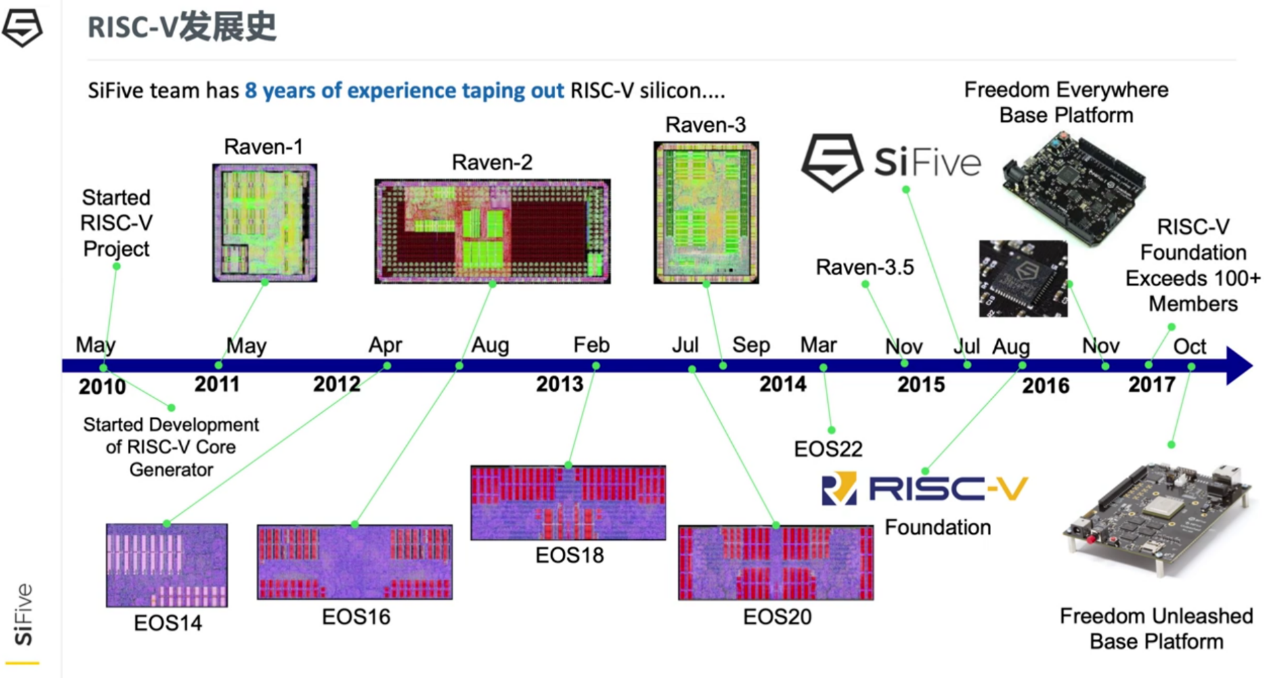
\includegraphics[scale=0.7]{img/one.png}
				\end{figure}
			\subsubsection{RISC-V指令简述}
				\begin{enumerate}
					\item 
						RSICV指令集分为基本指令集I和扩展指令集M,A,F,D,C。基本指令集I是整数指令集,也是RISC-V中,对于任何处理器必须有的指令集,扩展指令集可有可无。
						\begin{figure}[H]
							\centering
							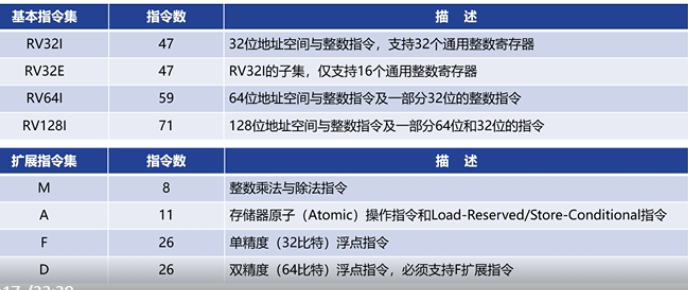
\includegraphics[scale=0.6]{img/two.png}
						\end{figure}
					\item
						基本指令集有六种格式:
					\begin{enumerate}		
						\item 
							R 类型指令:用于寄存器 - 寄存器操作;
						\item 
							I 类型指令:用于短立即数和访存 load 操作;
						\item 
							S 类型指令:用于访存 store 操作;
						\item 
							B 类型指令:用于条件跳转操作;
						\item 
							U 类型指令:用于长立即数操作;
						\item 
							J 类型指令:用于无条件操作;
					\end{enumerate}
					\begin{figure}[H]
						\centering
						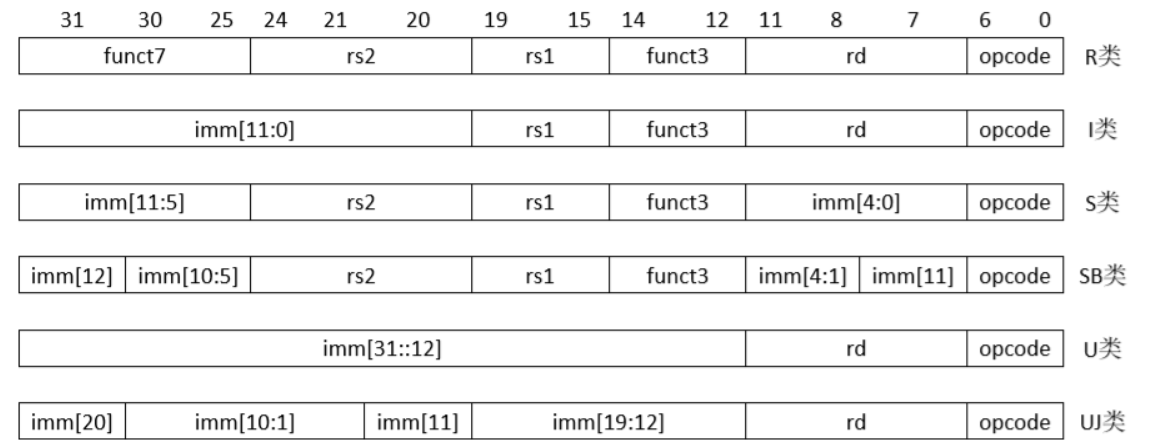
\includegraphics[scale=0.5]{img/three.png}
					\end{figure}
				\end{enumerate}
			\subsubsection{RISC-V指令分述}
			\begin{enumerate}
				\item{R型指令:}
					\begin{enumerate}
						\item{简介:}
							\subitem
								R型指令包含简单的运算指令,由两个32位源寄存器(rs1,rs2)进行运算,
								得到的结果存入一个32位目的寄存器(rd)。R型指令的6位操作码(opcode)
								是固定的,由功能码(func7和func3)确定是何种运算。
								\begin{figure}[H]
									\centering
									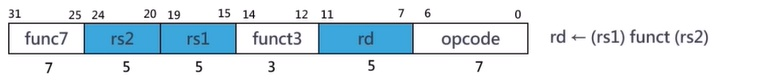
\includegraphics[scale=0.5]{img/r1.png}
								\end{figure}
						\item{数据通路\&指令执行流程:}
							\begin{figure}[H]
								\centering
								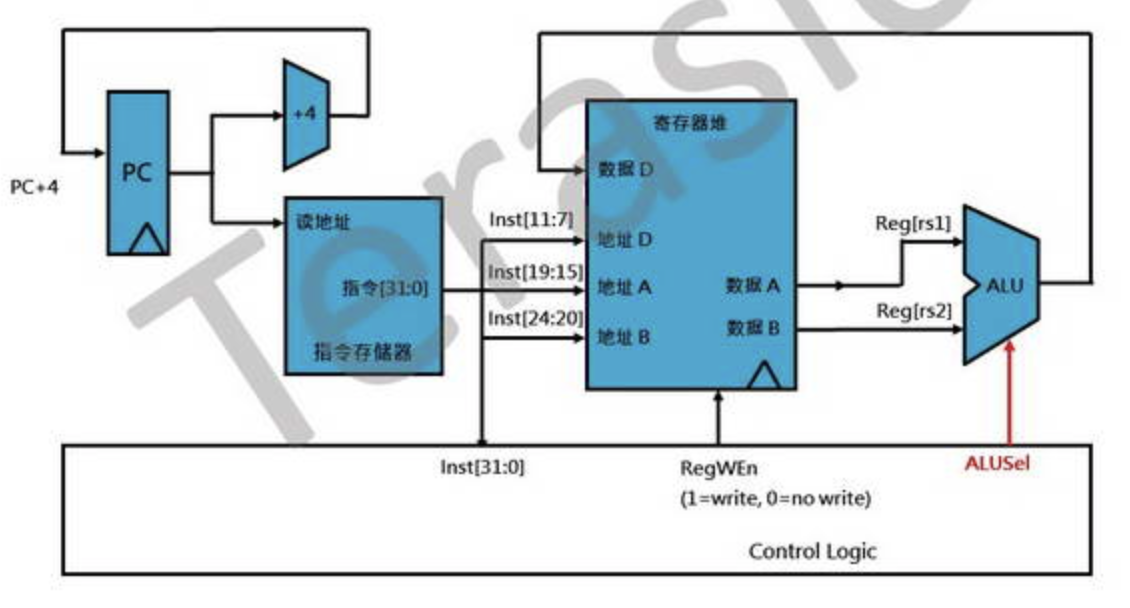
\includegraphics[scale=0.5]{img/r2.png}
							\end{figure}
							\begin{enumerate}
								\item
									首先按照PC中的地址,从指令存储器中读出32位指令,然后PC+4;
								\item
									指令被送入控制器,控制器根据功能码和操作码确定这是R型指令中的某一条指令,并产生控制信号ALUSel和RegWEn;
								\item
									将指令的rs1、rs2、rd字段分别送到寄存器堆的相应地址端,寄存器根据rs1和rs2字段的地址读出对应的寄存器的值Reg[rs1]和Reg[rs2];
								\item
									ALU根据控制信号ALUSel,对Reg[rs1]和Reg[rs2]进行相应的运算,得到运算结果;
								\item
									将运算结果送到寄存器堆的数据D端口,控制器产生的RegWEn信号使寄存器堆允许写入,寄存器堆根据地址D端口的地址将数据D端口的值写入相应的寄存器。
							\end{enumerate}
						\item{指令格式:}
							\begin{figure}[H]
								\centering
								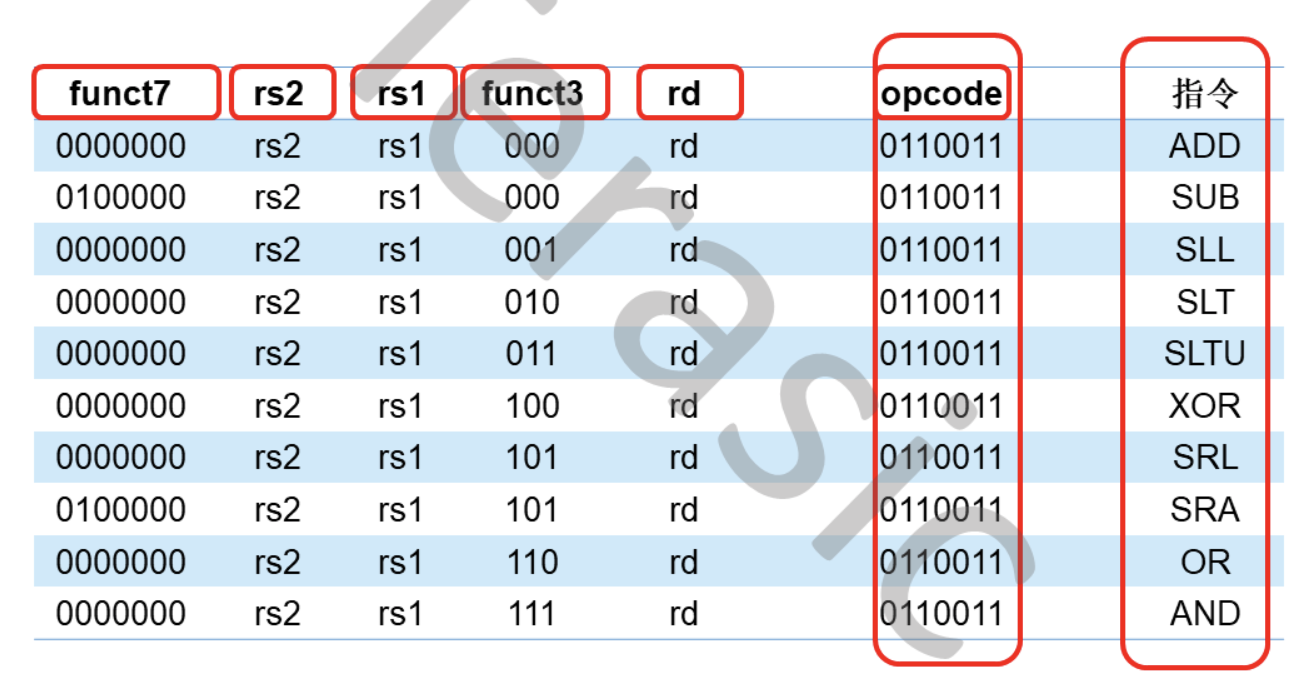
\includegraphics[scale=0.5]{img/r3.png}
							\end{figure}
							\begin{figure}[H]
								\centering
								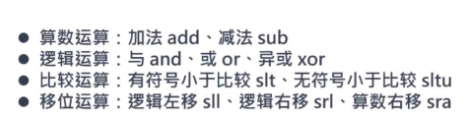
\includegraphics[scale=0.6]{img/r4.png}
							\end{figure}
					\end{enumerate}
				\item{I型指令:}
					\begin{enumerate}
						\item{简介:}
							\subitem
								I型指令包含简单的立即数运算指令和load指令。立即数运算指令是由一个32位源寄存器
								(rs1)和指令中包含的立即数(经扩充后的)进行运算,将得到的结果存入一个32位目的
								寄存器(rd)。I型指令中的立即数运算指令的6位操作码(opcode)固定,由功能码
								(func7和func3)确定是何种运算。
								\begin{figure}[H]
									\centering
									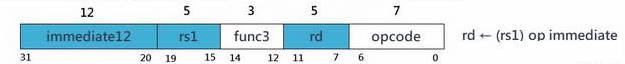
\includegraphics[scale=0.5]{img/i1.png}
								\end{figure}
							\subitem
								Load指令属于 I - type 型,其功能是完成存储器的读操作。
								funct3字段表示读出存储器的数据的字长(32位、16位或8位)。
								Load指令将rs1中的数据与12位立即数字段符号扩展相加所得到的结果
								作为访问存储器的地址,即存储器地址 = Reg[rs1] + imm。接着,
								将从存储器读出的数据存入目的寄存器rd中。
								\begin{figure}[H]
									\centering
									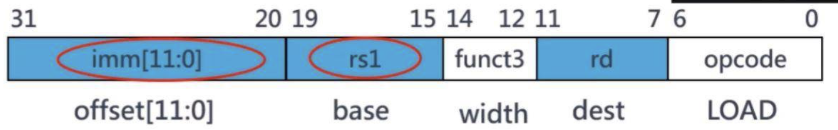
\includegraphics[scale=0.5]{img/il1.png}
								\end{figure}
						\item{数据通路\&指令执行流程:}
							\begin{figure}[H]
								\centering
								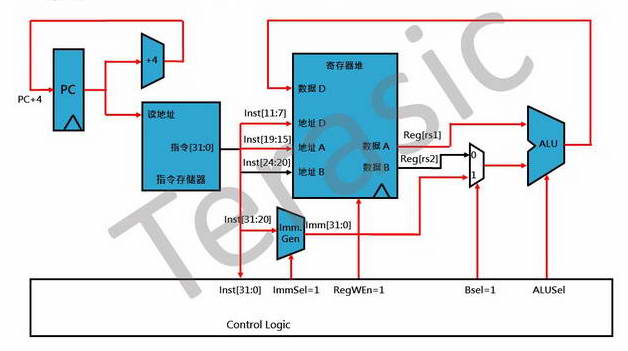
\includegraphics[scale=0.5]{img/i2.png}
							\end{figure}
							\begin{enumerate}
								\item
									首先按照PC中的地址,从指令存储器中读出32位指令,然后PC+4;
								\item
									指令被送入控制器,控制器根据功能码和操作码确定这是I型指令中的某一条指令,并产生控制信号ALUSel、ImmSel和RegWEn;
								\item
									将指令的rs1、rs2、rd字段分别送到寄存器堆的相应地址端,寄存器根据rs1和rs2
									字段的地址读出对应的寄存器的值Reg[rs1]和Reg[rs2](但此时Reg[rs2]没有用);
								\item
									将指令的12位立即数字段送到立即数扩展电路,通过ImmSel信号的指示,将立即数扩展为32位,并送到多路选择器的一个端口;
								\item
									Bsel信号,控制多路选择器选择立即数的那个端口,将立即数传送到ALU的一个输入端;
								\item
									ALU根据控制信号ALUSel,对Reg[rs1]和扩展后的立即数进行相应运算,得到运算结果;
								\item
									将运算结果送到寄存器堆的数据D端口,寄存器堆根据地址D端口的值将运算结果写入相应的寄存器。
							\end{enumerate}
						\item{指令格式:}
							\begin{figure}[H]
								\centering
								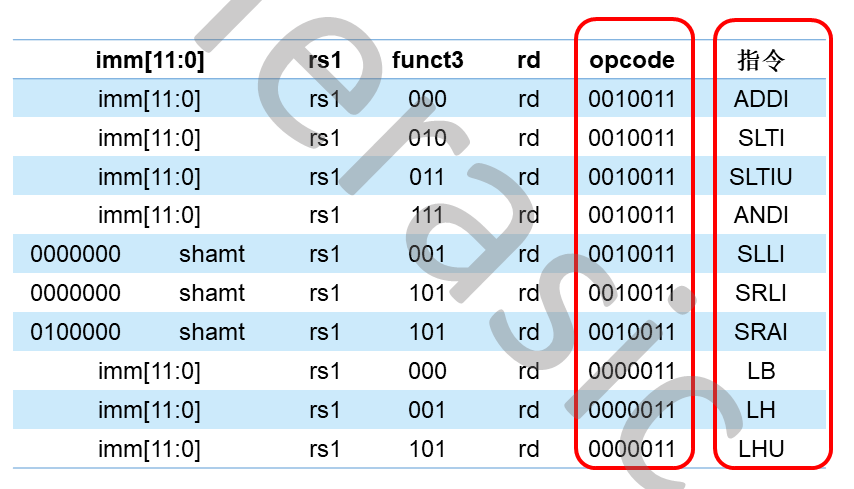
\includegraphics[scale=0.5]{img/i3.png}
							\end{figure}
							\begin{figure}[H]
								\centering
								
\includegraphics[scale=0.6]{img/i4.png}
							\end{figure}
					\end{enumerate}
				\item{S型指令:}
					\begin{enumerate}
						\item{简介:}
							\subitem
							S - type型指令包括Store 指令,其功能是完成存储器的写操作。
							Store使用funct3字段选择Word,HalfWord,Byte。
							Store指令将rs1中的数据与12位立即数字段符号扩展相加所得到的结果
							作为访问存储器的地址,即存储器地址 = Reg[rs1] + imm。接着,将
							rs2中的数据写入存储器相应地址中。
								\begin{figure}[H]
									\centering
									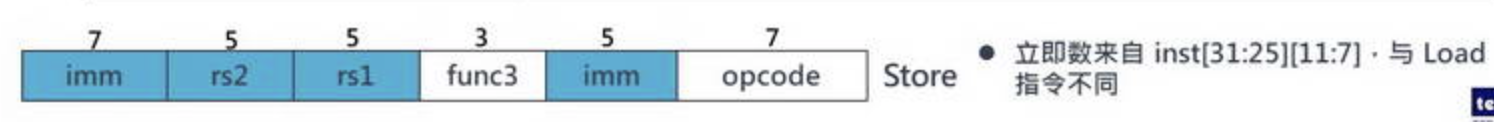
\includegraphics[scale=0.5]{img/s1.png}
								\end{figure}
						\item{数据通路\&指令执行流程:}
							\begin{figure}[H]
								\centering
								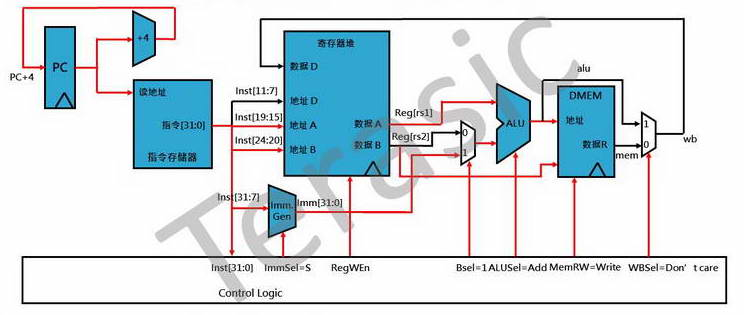
\includegraphics[scale=0.5]{img/s2.png}
							\end{figure}
							\begin{enumerate}
								\item
									首先按照PC中的地址,从指令存储器中读出32位指令,然后PC+4;
								\item
									指令中的控制码和功能码送到控制器中产生相应的控制信号;
								\item
									将rs1和rs2的地址送入寄存器堆,得到rs1寄存器的值Reg[rs1],作为ALU的第一个输入端;rs2寄存器的值Reg[rs2],作为DMEM写入地址的数据;
								\item
									将12位的立即数进行符号扩展,得到32位的立即数作为ALU的第二个输入端。此处控制信号Bsel=1,表示指令的立即数部分有效,二选一选择器输出立即数的内容;
								\item
									控制信号ALUSel = Add,指示ALU做加法运算,得到的地址送入数据存储器DMEM的地址接口,并注意此时控制信号MemRW = Write,使得数据存储器处于写状态;
								\item 
									DMEM接收到地址和数据后,将所选地址空间写入Reg[rs2]。
							\end{enumerate}
						\item{指令格式:}
							\begin{figure}[H]
								\centering
								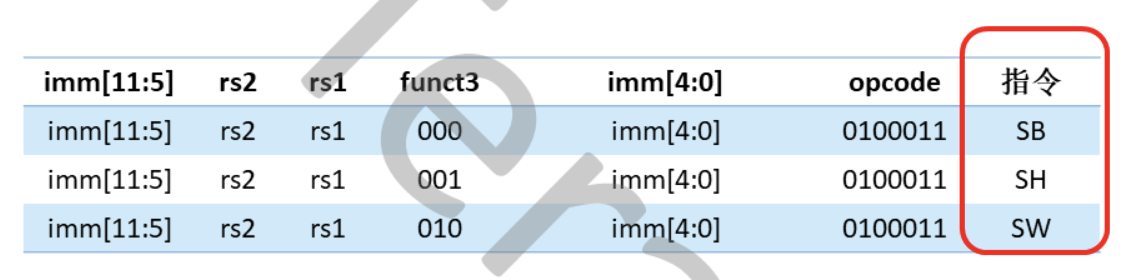
\includegraphics[scale=0.5]{img/s3.png}
							\end{figure}
					\end{enumerate}
				\item{B型指令:}
					\begin{enumerate}
						\item{简介:}
							\subitem
								B型指令的功能是比较寄存器rs1、rs2中的值,并根比较结果进行分支跳转。
								funct3字段表示分支跳转的类型。B型指令中beq/bne需进行相等比较的计
								算,blt/bltu与bge/bgeu需进行量值比较的计算。
								\begin{figure}[H]
									\centering
									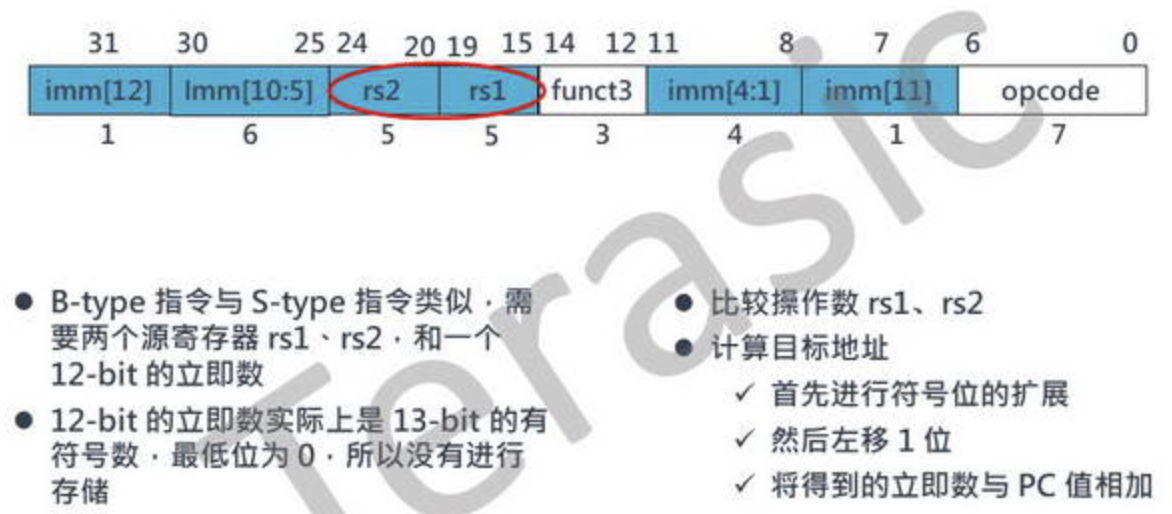
\includegraphics[scale=0.5]{img/b1.png}
								\end{figure}
						\item{数据通路\&指令执行流程:}
							\begin{figure}[H]
								\centering
								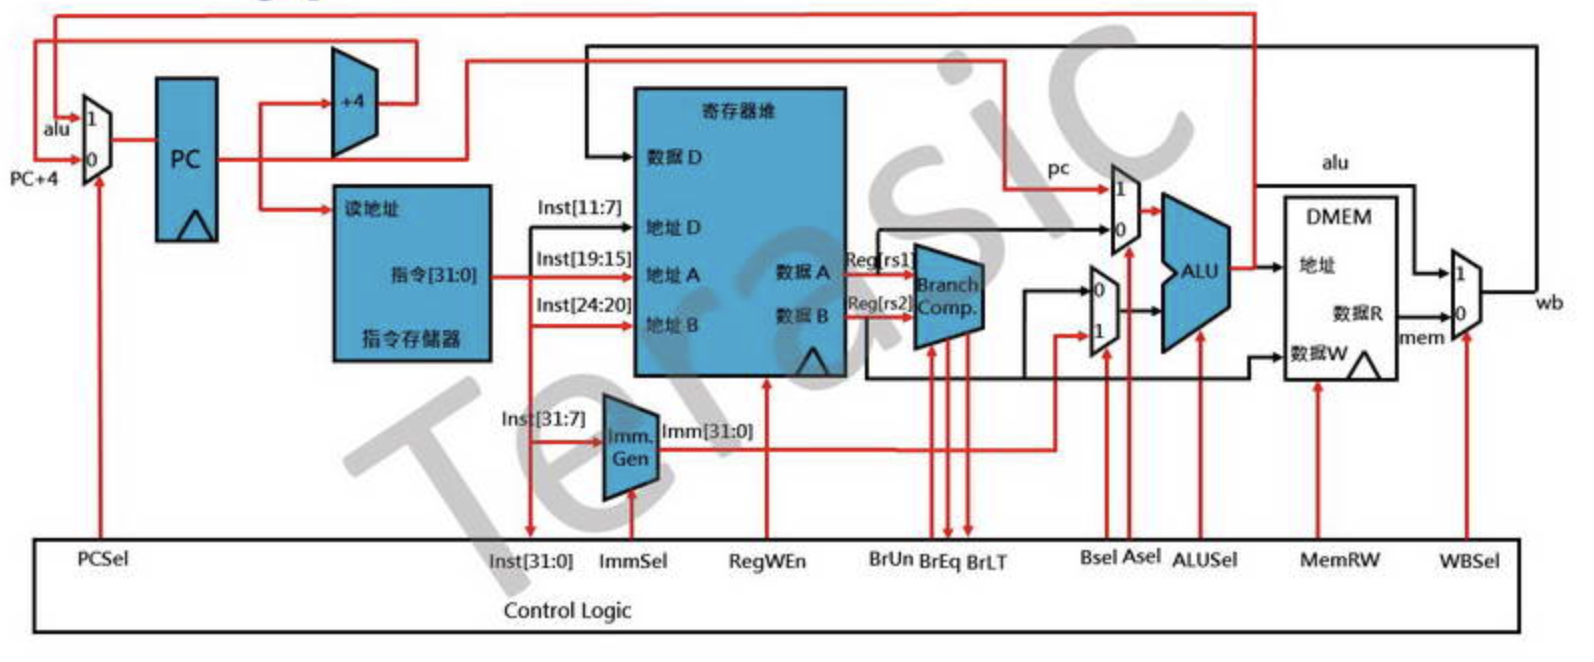
\includegraphics[scale=0.5]{img/b2.png}
							\end{figure}
							\begin{enumerate}
								\item
									首先按照PC中的地址,从指令存储器中读出32位指令,然后PC+4;
								\item
									指令中的控制码和功能码送到控制器中产生相应的控制信号;
								\item
									将指令中的rs1和rs2的地址送入寄存器堆,得到对应的寄存器的值Reg[rs1]和Reg[rs2];
								\item
									Reg[rs1]和Reg[rs2]被送入比较运算单元,比较后的结果送至控制器用于判断是否进行目标地址的跳转;
								\item
									将PC的值送至ALU的第一个输入端;
								\item
									将指令中的立即数字段送入立即数扩展电路,该电路输出一个32位的数,送至ALU的第二个输入端;
								\item
									若进行跳转,则由ALU计算出目标地址送至PC处。
							\end{enumerate}
						\item{指令格式:}
							\begin{figure}[H]
								\centering
								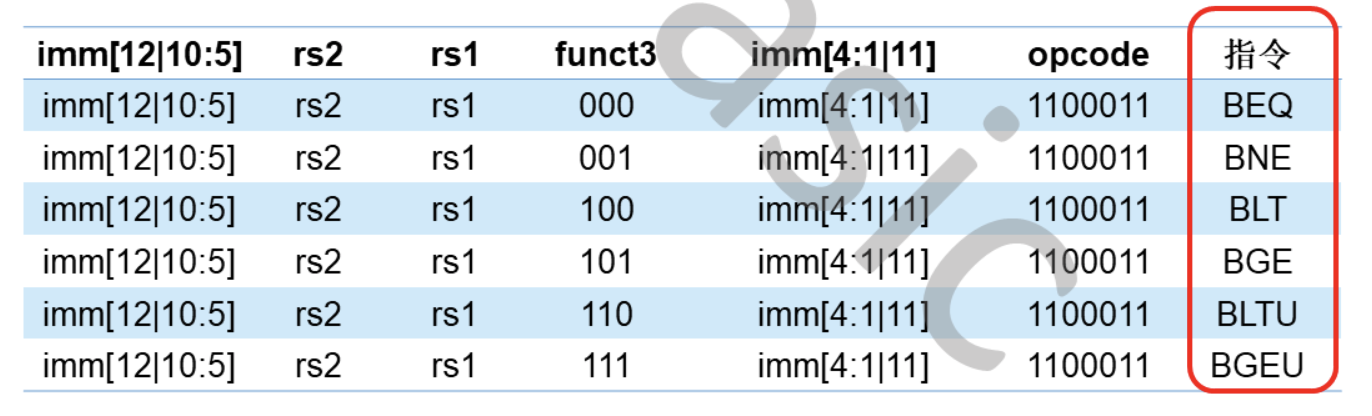
\includegraphics[scale=0.5]{img/b3.png}
							\end{figure}
					\end{enumerate}
				\item{U型指令:}
					\begin{enumerate}
						\item{简介:}
							\subitem
								U型指令包含LUI和AUIPC,用于构建32位常数,由20位立即数,rd和操作码构成。
								\begin{figure}[H]
									\centering
									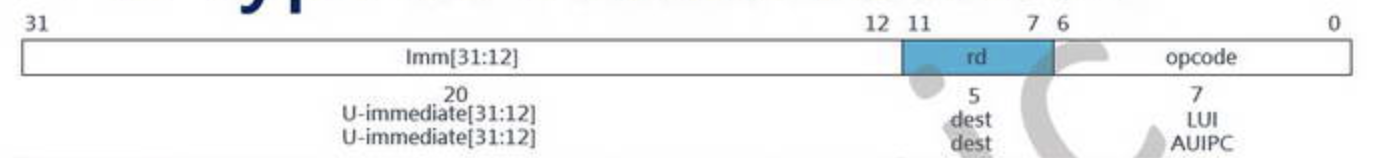
\includegraphics[scale=0.5]{img/u1.png}
								\end{figure}
						\item{数据通路\&指令执行流程:}
							\begin{figure}[H]
								\centering
								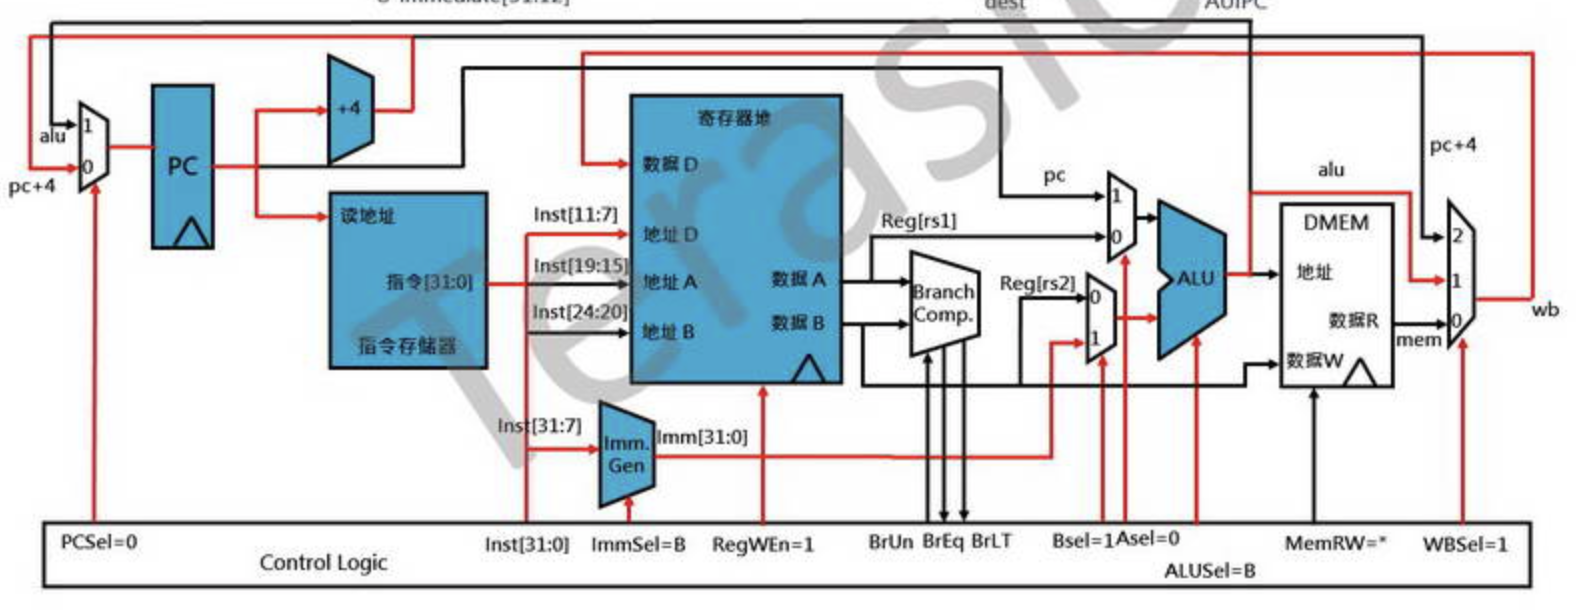
\includegraphics[scale=0.5]{img/u2.png}
							\end{figure}
							\begin{enumerate}
								\item
									首先按照PC中的地址,从指令存储器中读出32位指令,然后PC+4;
								\item
									指令中的控制码和功能码送到控制器中产生相应的控制信号;
								\item
									Bsel = 1使得ALU B端口输入扩展后的立即数,Asel = 1使得ALU A端口输入PC;
								\item
									将20位的立即数进行扩展(低12位填0),输入进ALU B端口;
								\item
									若是LUI指令,ALUsel = B(输出等于B端口输入);若是AUIPC指令, ALUsel = Add(将扩展后的立即数与PC相加);
								\item
									WBsel = 1使得ALU运算结果直接存入寄存器堆中rd所指寄存器;
							\end{enumerate}
						\item{指令格式:}
							\begin{figure}[H]
								\centering
								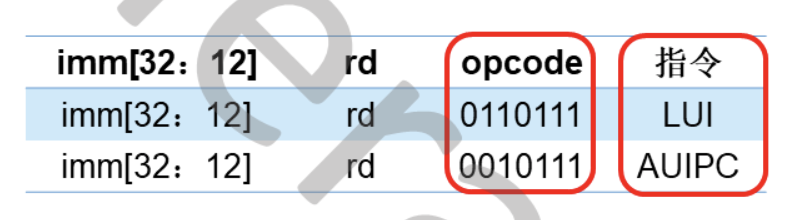
\includegraphics[scale=0.5]{img/u3.png}
							\end{figure}
					\end{enumerate}
				\item{J型指令:}
					\begin{enumerate}
						\item{简介:}
							\subitem
								JAL/JALR的功能是无条件跳转到目标地址。其中JAL指令中目标地址为PC的值加上20位的立即数所表示的偏移量,JALR指令中目标地址为寄存器rs1的值加上12位的立即数所表示的偏移量。
								JAL/JALR所需的计算类型只有加法运算。
								\begin{figure}[H]
									\centering
									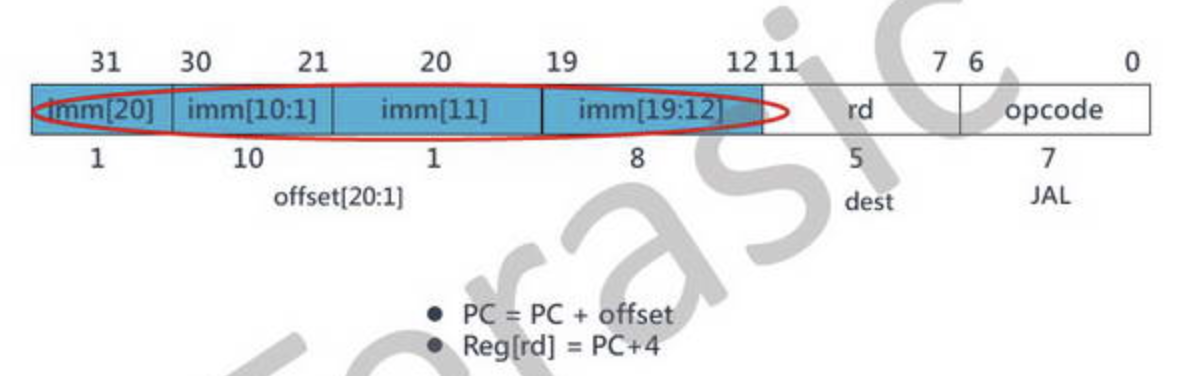
\includegraphics[scale=0.5]{img/j11.png}
								\end{figure}
								\begin{figure}[H]
									\centering
									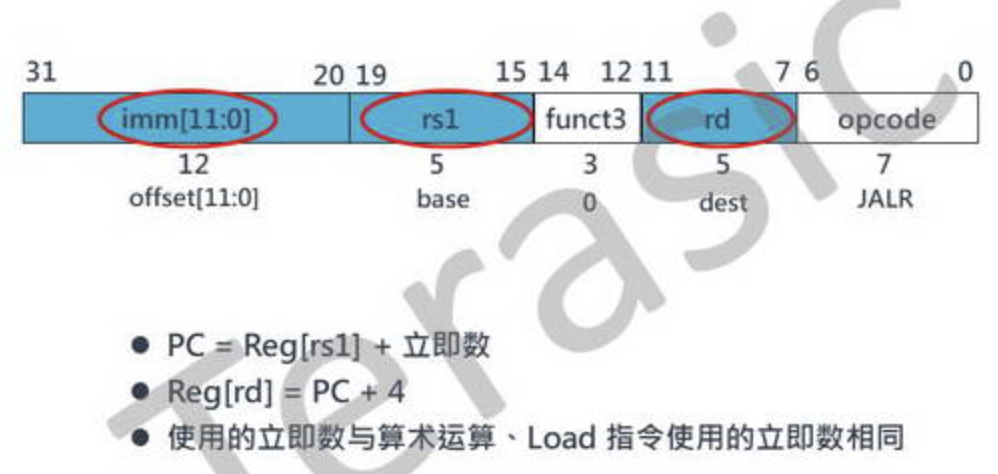
\includegraphics[scale=0.5]{img/j12.png}
								\end{figure}
						\item{数据通路\&指令执行流程:}
							\subitem
								JAL
							\begin{figure}[H]
								\centering
								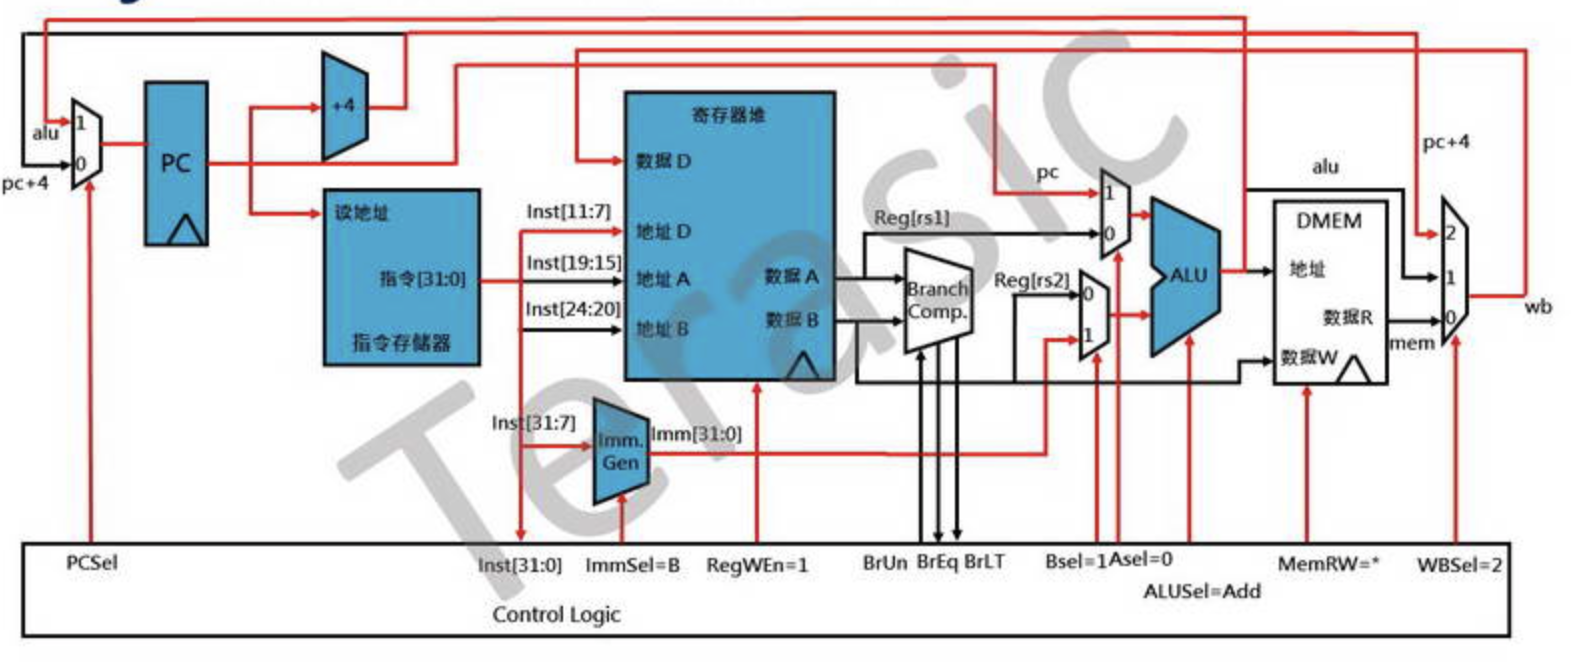
\includegraphics[scale=0.5]{img/j21.png}
							\end{figure}
							\begin{enumerate}
								\item
									首先按照PC中的地址,从指令存储器中读出32位指令,然后PC+4;
								\item
									指令中的控制码和功能码送到控制器中产生相应的控制信号;
								\item
									将PC的值送至ALU的第一个输入端;
								\item
									将指令中的立即数字段送入立即数扩展电路,该电路输出一个32位的数,送至ALU的第二个输入端;
								\item
									控制信号ALUSel = Add,指示ALU做加法运算,得到的结果即为目标地址,将其送至PC;
								\item 
									将原来PC+4的值写回到寄存器rd中;	
							\end{enumerate}
							\subitem
								JALR
							\begin{figure}[H]
								\centering
								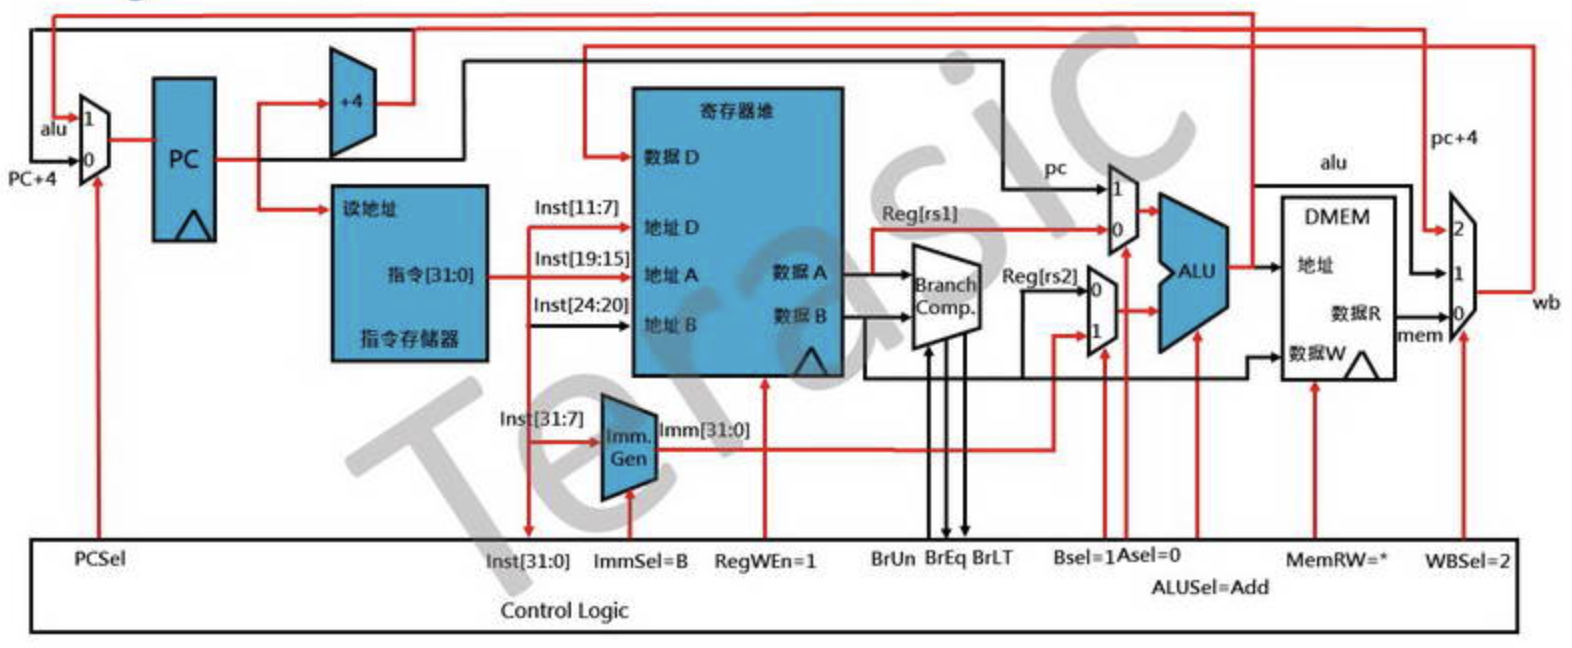
\includegraphics[scale=0.5]{img/j22.png}
							\end{figure}
							\begin{enumerate}
								\item
									首先按照PC中的地址,从指令存储器中读出32位指令,然后PC+4;
								\item
									指令中的控制码和功能码送到控制器中产生相应的控制信号;
								\item
									将指令中的rs1,rd的地址送入寄存器堆,得到rs1对应的寄存器的值Reg[rs1],并送入ALU的第一个端口;
								\item
									将指令中的立即数字段送入立即数扩展电路,该电路输出一个32位的数,送至ALU的第二个输入端;
								\item
									控制信号ALUSel = Add,指示ALU做加法运算,得到的结果即为目标地址,将其送至PC;
								\item 
									将原来PC+4的值写回到寄存器rd中;	
							\end{enumerate}
						\item{指令格式:}
							\begin{figure}[H]
								\centering
								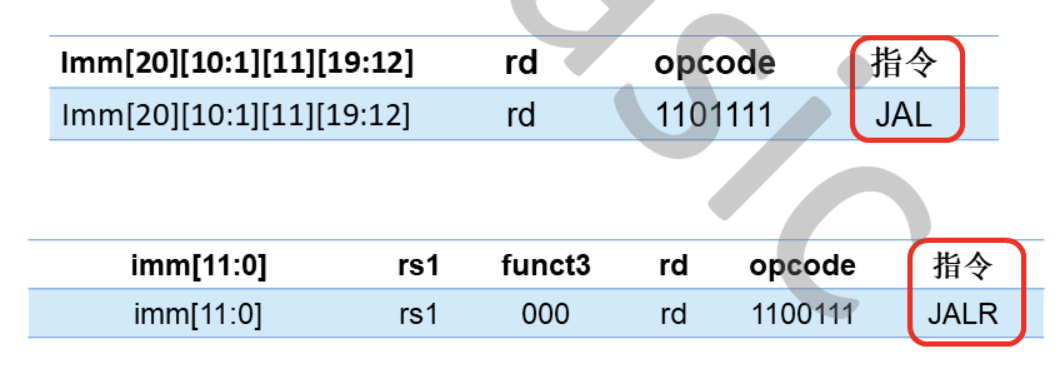
\includegraphics[scale=0.5]{img/j3.png}
							\end{figure}
					\end{enumerate}
			\end{enumerate}

		\subsection{蜂鸟E203简介}
			\subsubsection{E203}
				\begin{enumerate}
					\item 
						蜂鸟 E203 系列处理器由作者所在的公司开发,是一款开源的 RISC-V 处理器。蜂鸟是世
						界上最小的鸟类,其体积虽小,却有着极高的速度与敏锐度,可以说是“能效比”最高的鸟类。
						E203 系列以蜂鸟命名便寓意于此,旨在将其打造成为一款世界上最高能效比的 RISC 处理器。
				\end{enumerate}	
				\begin{figure}[H]
					\centering
					
\includegraphics[scale=0.8]{img/four.png}
				\end{figure}
					
			\subsubsection{E203 核心数据通路的模块划分}
				\begin{enumerate}
					\item 
						IFU 取址单元
					\item 
						EXU 执行单元
					\item 
						LSU 访存单元
					\item 
						BIU 总线
				\end{enumerate}	

			\subsubsection{E203 Core 的代码架构}
				\begin{figure}[H]
					\centering
					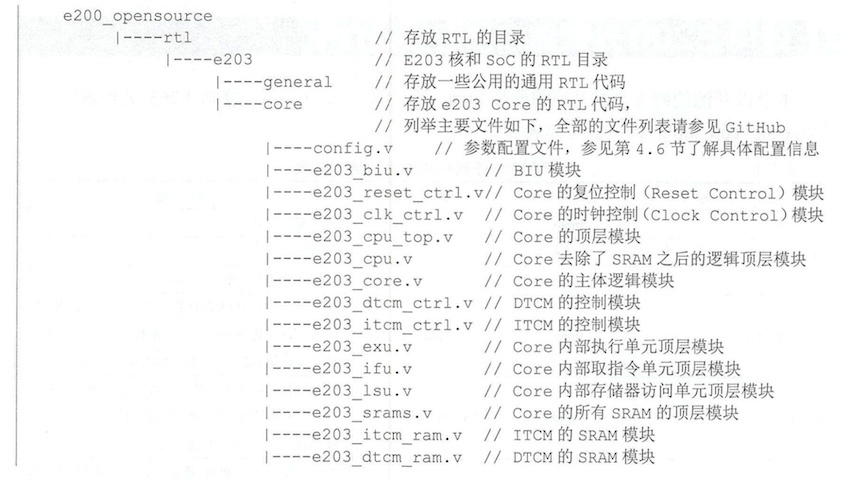
\includegraphics[scale=0.5]{img/framework.png}   
				\end{figure}

			\subsubsection{E203 数据通路的两级流程水线}
				\begin{enumerate}
					\item 
						第一级是IFU,包括,取址、分支预测、生成PC。
					\item 
						第二级是译码、派遣、执行、访存、写回。
				\end{enumerate}	

			\subsubsection{E203 的特点}
				\begin{enumerate}
					\item 
						蜂鸟E203 处理器研发团队拥有在国际一流公司多年开发处理器的经验,使用稳健的。
					\item 
						蜂鸟E203 的代码为人工编写,添加丰富的注释且可读性强,非常易于理解。
					\item 
						蜂鸟E203 专为IoT 领域量身定做,其具有2 级流水线深度,功耗和性能指标均优于目前主流商用的ARM Cortex-M 系列处理器,且免费开源,能够在IoT 领域完美替代ARM Cortex-M 处理器。
				\end{enumerate}	

		\subsection{T-core开发板介绍}
			\begin{enumerate}
				\item 
					T-core开发板是友晶科技公司的基于RISC-V的新款开发板。T-Core提供了围绕Intel MAX 10 FPGA构建的强大的硬件设计平台。它配备完善,可在控制平面或数据路径应用中提供具有成本效益的单芯片解决方案,并提供行业领先的可编程逻辑,以实现最终的设计灵活性。
				\item 
					借助MAX 10 FPGA,可以获得比上一代更低的功耗/成本和更高的性能。可支持大量应用,包括协议桥接,电机控制驱动,模数转换和手持设备。T-Core开发板包括硬件,例如板载USB-Blaster II,QSPI Flash,ADC接头连接器,WS2812B RGB LED和2x6 TMD扩展接头连接器。通过利用所有这些功能,T-Core是展示,评估和原型化Intel MAX 10 FPGA真正潜力的理想解决方案。T-Core还通过板载JTAG调试支持RISC-V CPU。它是学习RISC-V CPU设计或嵌入式系统设计的理想平台。
			\end{enumerate}	
			\begin{figure}[H]
				\centering
				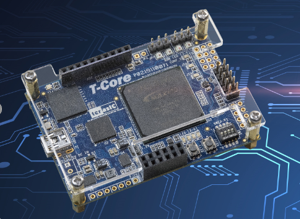
\includegraphics[scale=1]{img/five.png}
			\end{figure}
			\begin{figure}[H]
				\centering
				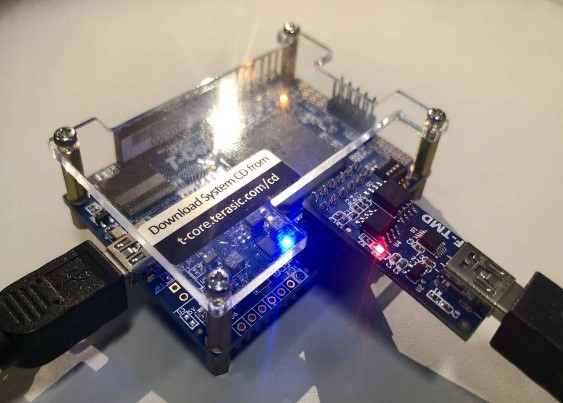
\includegraphics[scale=1]{img/six.jpg}
			\end{figure}

		\subsection{矩阵乘法运算指令及数据通路}
		\begin{enumerate}
			\item 常规矩阵运算与自定义矩阵乘法指令的对比
				\begin{itemize}
					\item{以 1 x 4 与 4 x 1 大小的矩阵相乘为例}
						\begin{figure}[H]
							\centering
							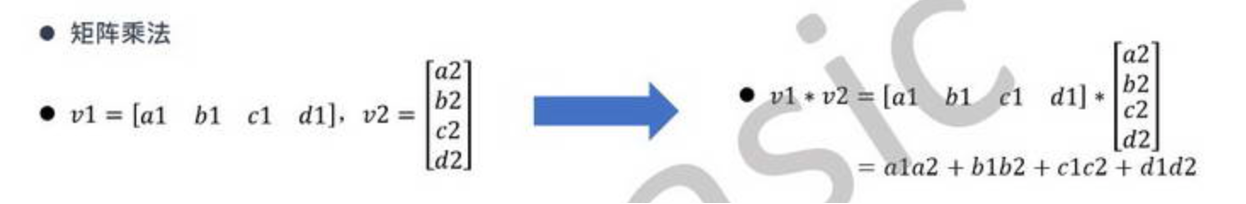
\includegraphics[scale=0.5]{img/dot1.png}
						\end{figure}
					\item{常规计算需要的总周期数:71;DOT 指令需要的总周期数:1\\}
						\begin{figure}[H]
							\centering
							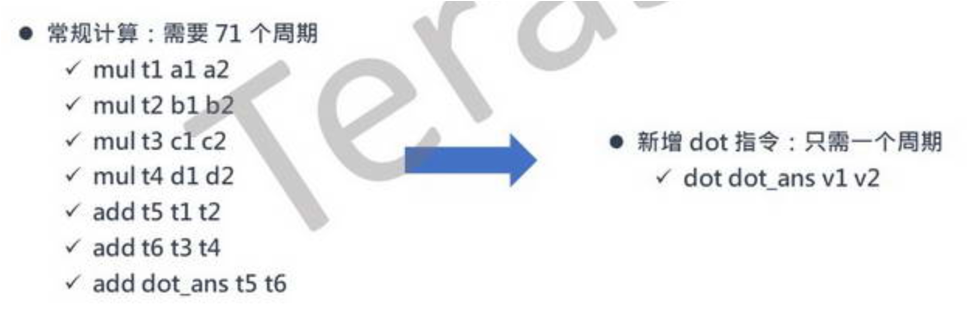
\includegraphics[scale=0.5]{img/dot2.png}
						\end{figure}
						(每条乘法指令:17个周期; 每条加法指令:1个周期)
				\end{itemize}

			\item DOT 指令格式\\
			操作码字段(opcode)选用 1101011;将功能字段(funct3)定义为 000,
			将 funct7 字段定义为 0000001;rs1 rs2 字段分别表示两个源操作数寄存器,
			rd 字段表示目标寄存 器。(注:在实际运算的时候,rs1、rs2 是没有被使用到的)。
				\begin{figure}[H]
					\centering
					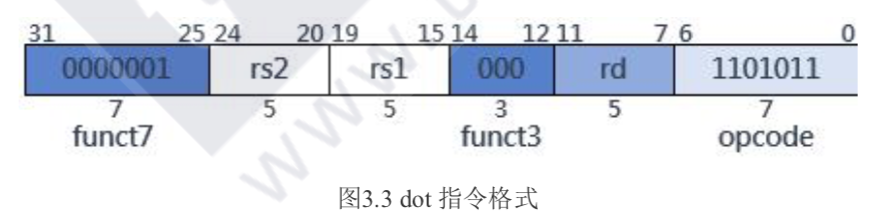
\includegraphics[scale=0.5]{img/dot3.png}
				\end{figure}
			
			\item DOT 指令数据通路分析 \\
			通过在ALU数据通路中增加几条选择线,可以实现在ALU中添加自定义逻辑单元,并通过译码信号使ALU输出该单元的计算结果。
			\begin{figure}[H]
				\centering
				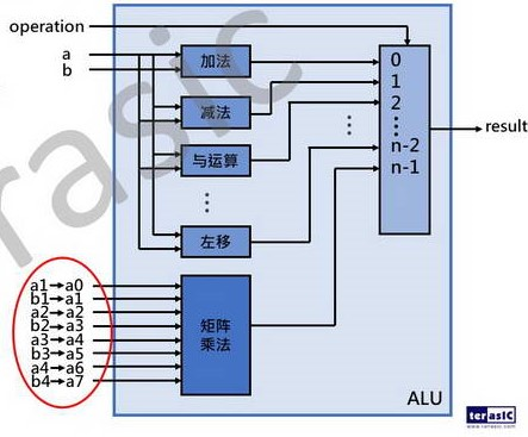
\includegraphics[scale=0.8]{img/alu2.png}
			\end{figure}
			\begin{figure}[H]
				\centering
				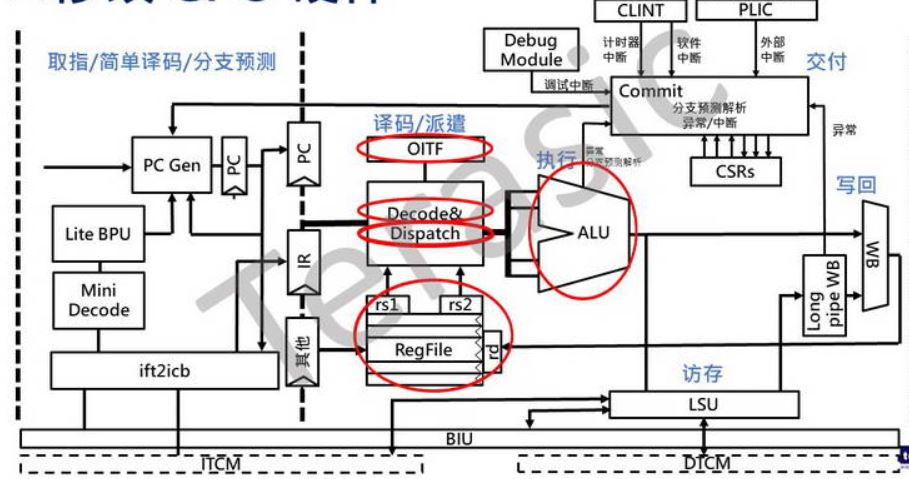
\includegraphics[scale=0.8]{img/datalink.jpg}
			\end{figure}
			\begin{itemize}
				\item RegFile:8个寄存器完成1,4 x 4,1的矩阵乘法空间,并与Dispatch模块建立读取通道
				\item Decode: 对指令进行译码
				\item Dispatch:增加dot指令相关的信号,将取得的数值传入ALU
				\item ALU:实现dot指令的实现
				\item OITF:解决寄存器与长指令的存取目的寄存器之间的冲突;同时Dispatch模块负责处理冲突后的操作
			\end{itemize}
		\end{enumerate}
		
		
	\section{实践篇}
	\subsection{硬件开发}
	我们在Quartus上通过Verilog语言对CPU中的EXU执行单元模块进行修改,修改的步骤大致分为以下几个方面:
	\begin{itemize}
		\item 增加DOT4、DOT3、DOT2指令的宏定义;
		\item 给出DOT4、DOT3、DOT2的译码条件,加入ALU运算集,连接ALU INFO总线;
		\item 声明a0-a7的端口,把这8个端口对应到x10-x17寄存器上;
		\item 如果OITF中有长指令正在维护并且要写回目的寄存器 x10-x17 中的话,那就有数据冒险,不可以派遣;
		\item 把传来八个寄存器转到ALU;
		\item 编写DOT4、DOT3、DOT2指令的ALU逻辑实现模块,并将得到的结果写回。
	\end{itemize}
	硬件修改的数据通路图如下图所示,我们将在红圈的地方进行增添和修改。
	\begin{figure}[H]
		\centering
		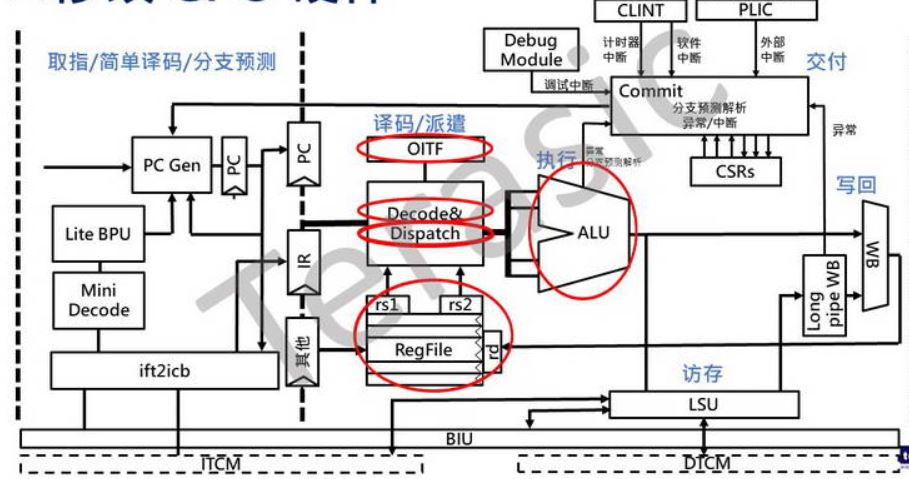
\includegraphics[scale=0.8]{img/datalink.jpg}
		\caption{硬件数据通路图及修改部分}
	\end{figure}
	\subsubsection{宏定义修改}
	为了增加ALU的多路选择数,我们在宏定义中增加三条选择线路,分别连接DOT4、DOT3、DOT2的自定义逻辑功能模块,对应的修改为将ALU的宏定义宽度加3:
	\begin{figure}[H]
		\centering
		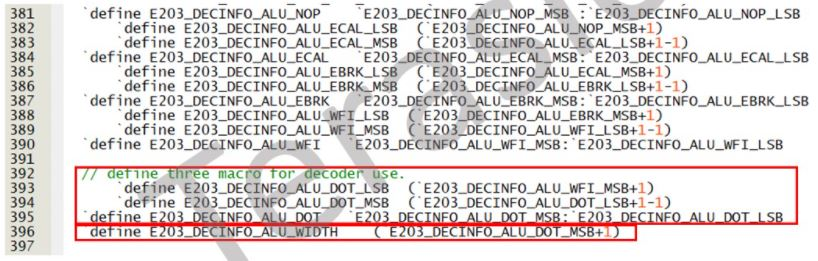
\includegraphics[scale=1]{img/define.jpg}
		\caption{宏定义修改说明}
	\end{figure}
	
	\subsubsection{译码模块修改}
	将DOT4、DOT3、DOT2的指令字段确定之后,给出其译码的条件,并将其放入ALU运算集合之中。之后还需将这三个指令的译码信息放入总线用于数据交换。
	\begin{figure}[H]
		\centering
		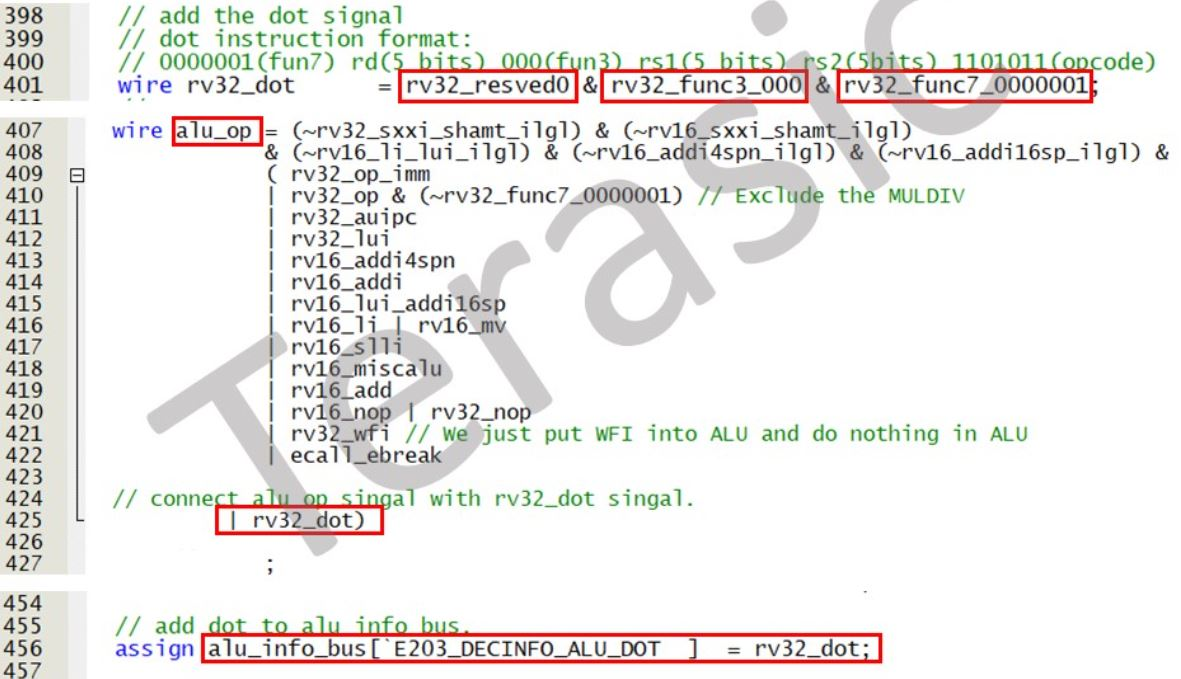
\includegraphics[scale=0.7]{img/decode.jpg}
		\caption{译码模块修改说明}
	\end{figure}
	
	\subsubsection{寄存器堆模块修改}
	该处的修改较为简单,主要工作是声明a0-a7这8个端口,并分别对应到寄存器堆中x10-x17这8个寄存器.这里需要强调一下,使用这8个寄存器是由于他们均为函数调用的传参寄存器,在运行过程中使用几率较小,所以产生冲突的可能性更小,从而保证更高的处理效率。
	\begin{figure}[H]
		\centering
		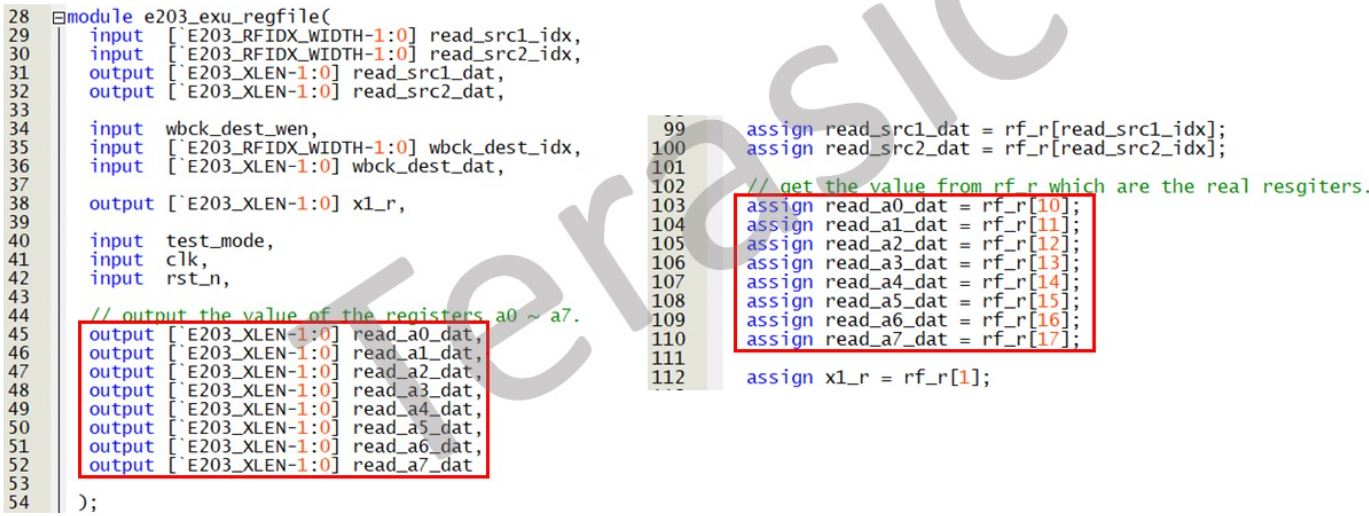
\includegraphics[scale=0.6]{img/register.jpg}
		\caption{寄存器堆修改说明}
	\end{figure}

	\subsubsection{OITF模块修改}
	e203解决结构冒险是用到了握手机制。用一个 op\_ready信号 \& op信号进行判断,若为1就可以派遣, 若不为1就不能派遣。若正在执行乘法,下一条还是乘法, 此时op\_ready就是0,op就是1,与后等于0,无法派遣。如果正在执行乘法,下一条是跳转指令 op\_ready就是1,op为1,与后等于1,可以派遣。
	
	运用这个机制,我们对我们所使用的8个寄存器进行冲突判断。在e203中,有一种特殊定义的长指令,在派遣后还需执行几个周期,访存相关的指令。e203在执行长指令的时候,OITF指令会把相关信息压入OITF中,执行完释放,这叫做维护或数据依赖性,维护期间如果来了一个非长指令,就很有可能冲突。所以OITF就是用来判断是否会发生长指令和非长指令的冲突。
	\begin{figure}[H]
		\centering
		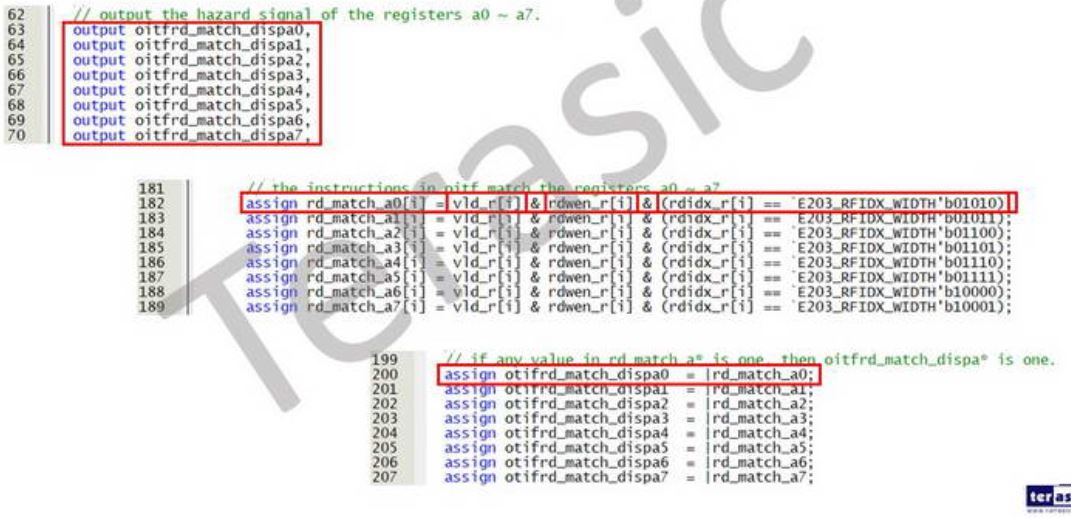
\includegraphics[scale=0.8]{img/OITF.jpg}
		\caption{OITF模块修改说明}
	\end{figure}
	
	\subsubsection{派遣模块修改}
	派遣模块需要修改两个部分,一个是针对OITF反馈的派遣信息的响应,一个是针对寄存器值派遣给ALU模块的赋值过程。
	\begin{figure}[H]
		\centering
		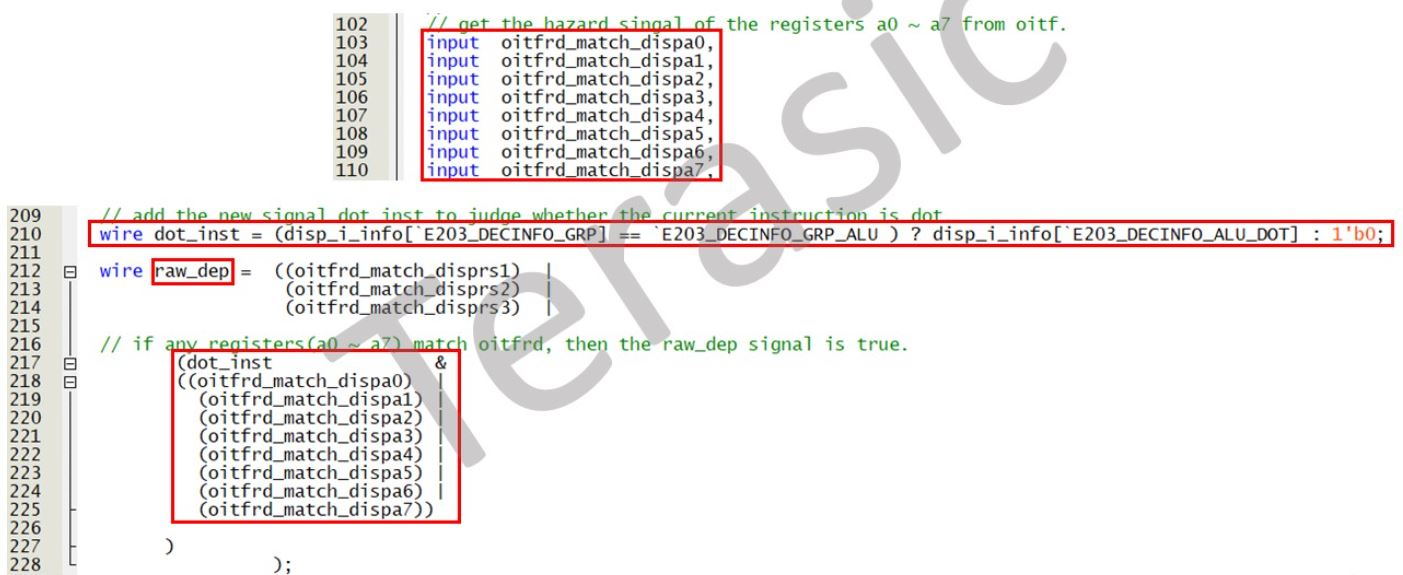
\includegraphics[scale=0.6]{img/dispatch1.jpg}
		\caption{OITF反馈的派遣信息的响应}
	\end{figure}
	\begin{figure}[H]
		\centering
		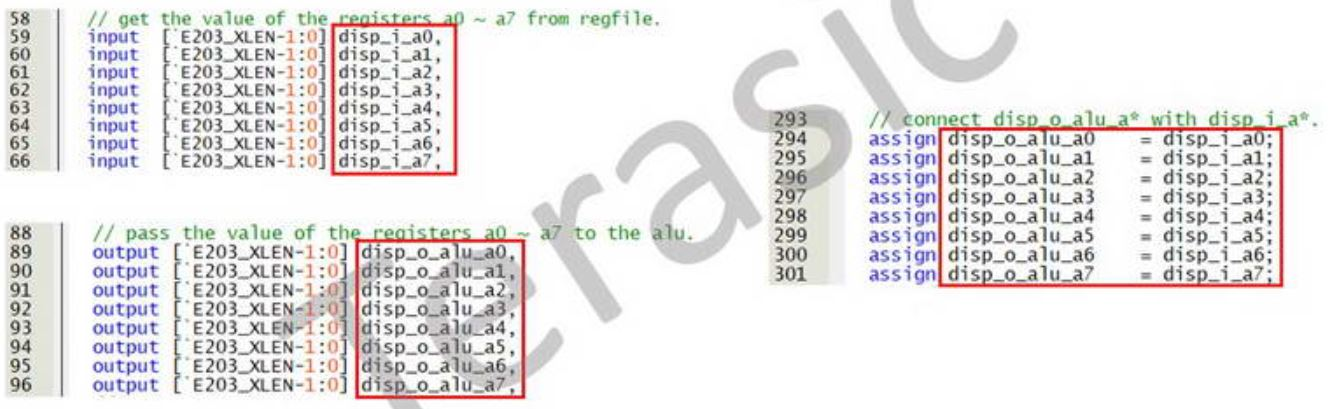
\includegraphics[scale=0.6]{img/dispatch2.jpg}
		\caption{寄存器值派遣给ALU模块的赋值过程}
	\end{figure}

	\subsubsection{ALU模块修改}
	首先需要接收到来自总线上关于DOT指令的控制信息,来指示ALU当前需要执行DOT指令的操作。接着我们在ALU的数据通路模块中增加自定义逻辑模块,将我们想实现的三种子块矩阵乘法写入相应位置中。在最后我们需要将ALU输出的结果存入相应的寄存器中,来保证结果被缓存而不被覆盖。
	\begin{figure}[H]
		\centering
		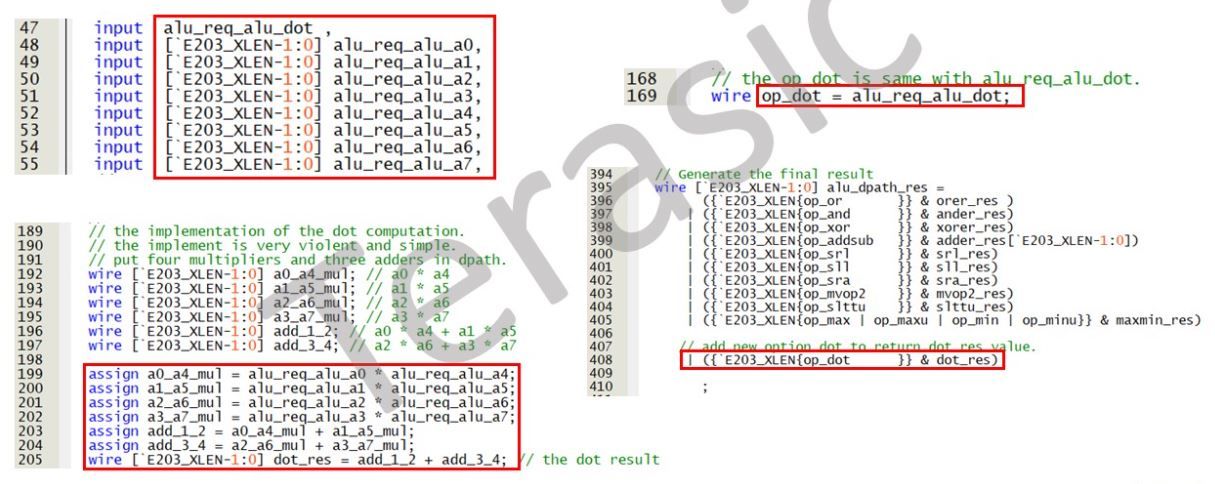
\includegraphics[scale=0.7]{img/alu.jpg}
		\caption{DOT4的自定义逻辑实现}
	\end{figure}

	以上便是所有硬件修改的流程,在完成修改之后,我们需要对Quartus工程项目进行编译,若编译成功,证明修改完全正确。编译之后会在outfile文件夹中得到pof文件,这个文件正是需要我们烧写进T-Core的文件。
	
	\subsubsection{烧写POF文件到T-Core开发板}
	\begin{itemize}
		\item 设置T-Core开发板的SW2开关:SW2.1=0,SW2.2=1。
		\begin{figure}[H]
			\centering
			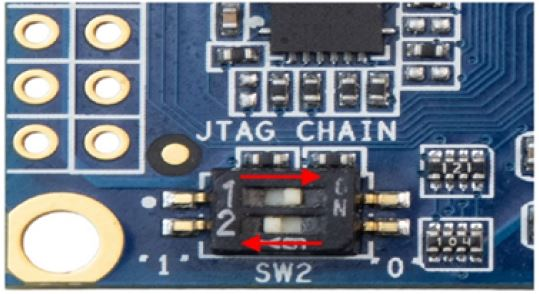
\includegraphics[scale=0.7]{img/jtag.jpg}
			\caption{JTAG 切换模式}
		\end{figure}
		\item 用Mini USB线连接T-Core开发板的J2接口与主机。
		\item 打开Quartus的Programmer工具, 点击Hardware Setup...,选择T-Core,然后点击Auto Detect。选择当前T-Core开发板的MAX 10 FPGA器件,点击change file按钮并选择刚刚生成好的POF文件,勾号选项之后点击start开始烧写。
		\begin{figure}[H]
			\centering
			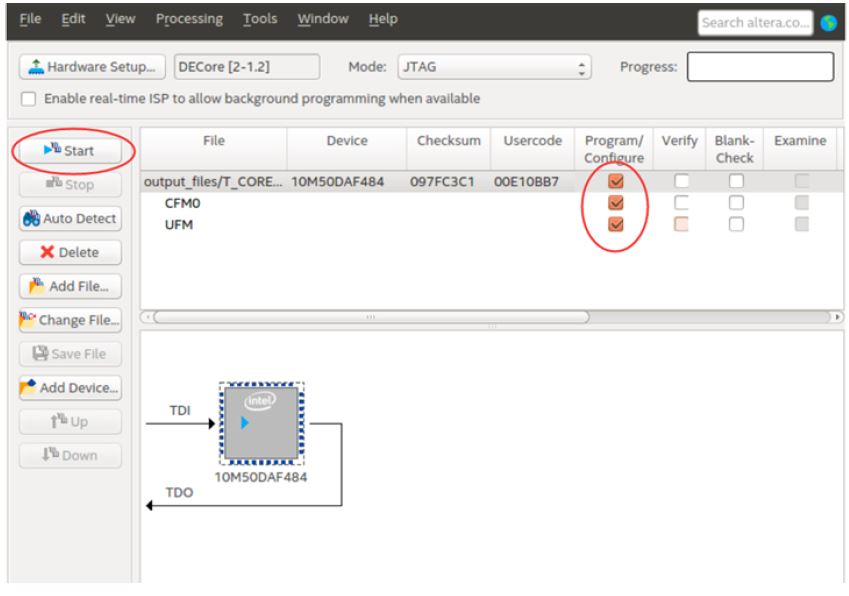
\includegraphics[scale=0.7]{img/pof.jpg}
			\caption{PROGRAMMER 界面操作一览}
		\end{figure}
		
	\end{itemize}	
	\subsection{软件开发}
	我们需要根据我们设计的指令格式修改编译器,使其能够编译dot指令,并将其转换为对应的机器码。这样,编译器就可以将包含dot指令的测试程序编译成可执行文件,供硬件执行。
	\subsubsection{生成操作码宏定义}
		\begin{itemize}
			\item 文件包riscv-opcodes中枚举了全部RISC-V指令的操作码信息。因为我们设计的dot指令属于rv32i指令集,因此需要在opcodes-rv32i文件中加入我们编写的dot指令的指令格式。
				\begin{figure}[H]
					\centering  
					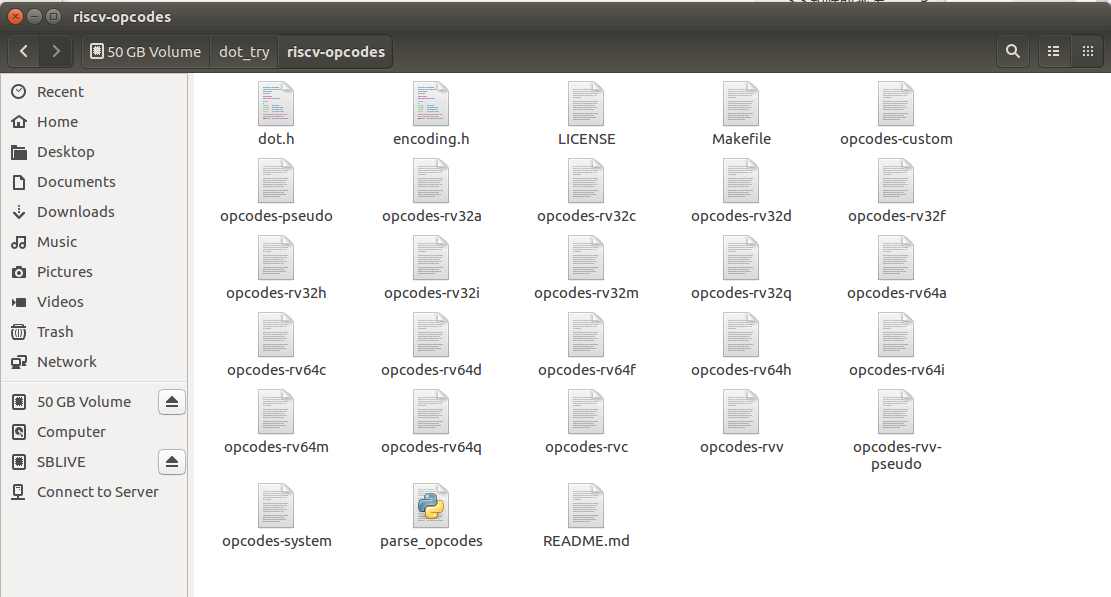
\includegraphics[scale=0.3]{img/1.png}   
					\caption{riscv-opcodes文件包}
				\end{figure}
				\begin{figure}[H]
					\centering  
					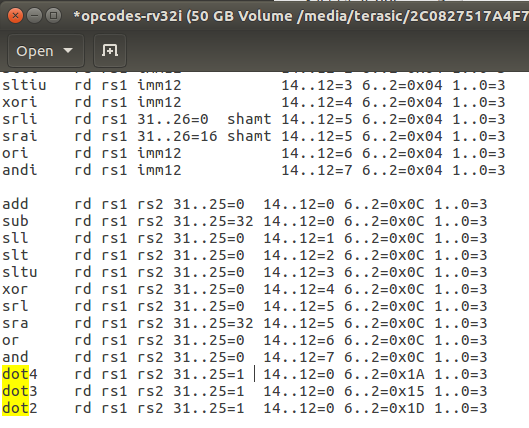
\includegraphics[scale=0.5]{img/2.png}   
					\caption{修改 opcodes-rv32i 文件}
				\end{figure}
			\item 运用转换脚本parse\_opcodes生成编译器所需要的信息,即C语言格式的宏定义,存放在dot.h中
				\begin{figure}[H]
					\centering  
					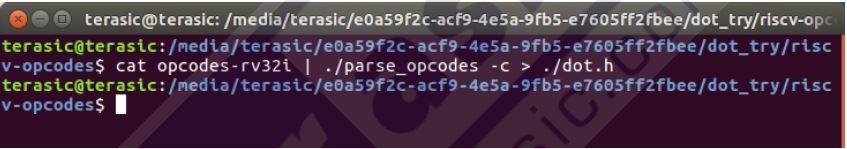
\includegraphics[scale=0.8]{img/changeopcodes.JPG} 
					\caption{用脚本转换 opcodes}
				\end{figure}
		\end{itemize}
	
		\subsubsection{修改 RISC-V GNU工具链}
		RISC-V GNU工具链是一组用于支持RISC-V C和C++的交叉编译工具链,这些工具构成了一个完整的系统。GNU工具链包括riscv-gcc、riscv-glibc等子仓库。
		\begin{itemize}
			\item 从gitee上下载完整的工具链后,打开 "riscv-gnu-toolchain/riscv-binutils/include/opcode" 路径下的 riscv-opc.h 文件,将第1步中生成的dot指令相关的定义和代码复制到该文件中。
				\begin{figure}[H]
					\centering  
					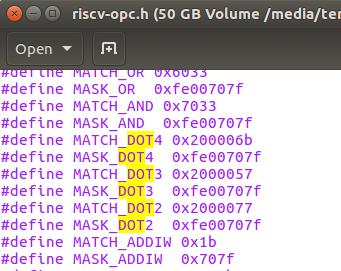
\includegraphics[scale=0.8]{img/3.png} 
					\caption{更改工具链}
				\end{figure}
				\begin{figure}[H]
					\centering   
					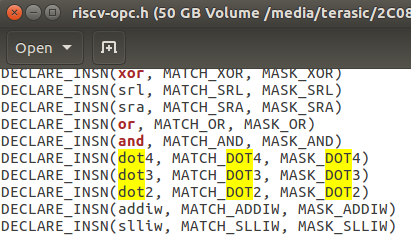
\includegraphics[scale=0.7]{img/4.png} 
					\caption{更改工具链}
				\end{figure}
			\item 打开 "riscv-gnu-toolchain/riscv-binutils/opcodes" 路径下的 riscv-opc.c 文件,找到定义的 riscv\_opcodes 结构体,在其中添加dot指令
				\begin{figure}[H]
					\centering  
					\includegraphics[scale=0.5]{img/5.png} 
					\caption{更改工具链}
				\end{figure}
			\item 修改完成后,我们需要安装一些编译依赖,然后就可以重新编译生成工具链了,此过程较长,需要20分钟左右。
				\begin{figure}[H]
					\centering  
					\includegraphics[scale=0.8]{img/COMPILE.JPG} 
					\caption{编译工具链}
				\end{figure}
		\end{itemize}
		
		\subsubsection{测试指令}
			\begin{itemize}
				\item 首先在 dot\_try 文件夹下新建一个 tool\_test
				文件夹,并在其中新建 dot.c 文件,用于测试 dot 指令是否可以被正常编译。
					\begin{figure}[H]
						\centering  
						\includegraphics[scale=0.6]{img/6.png} 
						\caption{编写测试程序}
					\end{figure}
				\item 调用 gcc 编译 dot.c 文件,如果成功修改了工具链,就会生成 dot 文件。
					\begin{figure}[H]
						\centering  
						\includegraphics[scale=0.8]{img/makedot.JPG} 
						\caption{调用 gcc 编译}
					\end{figure}
				\item 进行汇编代码查看。可以在 dot2\_test、dot3\_test、dot4\_test 函数的片段中,找到生成的 dot 汇编指令。
					\begin{figure}[H]
						\centering  
						\includegraphics[scale=0.7]{img/7.png} 
						\caption{查看 dot 指令}
					\end{figure}		
			\end{itemize}
		\subsubsection{创建程序文件}
		\begin{itemize}
			\item 在 "demo\_dot" 文件夹下创建一个 "demo\_dot.c" 的文本文档。包含以下头文件。
			\begin{lstlisting}[language={C++}]
				#include <stdio.h>
				#include <stdlib.h>
				#include <stdbool.h>
				#include <stdatomic.h>
				#include "encoding.h"
				#include <platform.h>  
			\end{lstlisting}
			\item 宏定义,三个常数 CONST\_I、CONST\_K、CONST\_J 分别为 32、64、32,定义标识符
			A\_ROW(矩阵 A 的行)为 CONST\_I,定义 A\_COL(矩阵 A 的列)为 CONST\_K;定义标识符
			B\_ROW(矩阵 B 的行)为 CONST\_K,定义 B\_COL(矩阵 B 的列)为 CONST\_J;定义标识符
			RES\_ROW(乘法运算得到的新矩阵的行)为 CONST\_I,定义 A\_COL(乘法运算得到的新矩阵的
			列)为 CONST\_J。
			\begin{lstlisting}[language={C++}]
				// matrix dimensions
				// CONST_K must set as multiple of 4 for dot instruction
				#define CONST_I 32
				#define CONST_K 64
				#define CONST_J 32
				//a[const_i][const_k]
				#define A_ROW CONST_I
				#define A_COL CONST_K
				//b[const_k][const_j]
				#define B_ROW CONST_K
				#define B_COL CONST_J
				//res[const_i][const_j]
				#define RES_ROW CONST_I
				#define RES_COL CONST_J  
			\end{lstlisting}
			\item 定义 demo\_uart\_init 函数,用于初始化,首先配置 GPIO\_IOF\_EN 对应的比特位为 1,使能 IOF 模
			式,再将 GPIO\_IOF\_SEL 对应的比特位清零,选择 IOF0,再配置 UART\_DIV 寄存器,设置波特
			率约为 115200。最后配置 UART\_TXCTRL 和UART\_RXCTRL,将 UART0 的 TX 和 RX 使能。
			\begin{lstlisting}[language={C++}]
				void uart_init(){
					// Configure UART to print
					GPIO_REG(GPIO_IOF_EN) |= IOF0_UART0_MASK;
					GPIO_REG(GPIO_IOF_SEL) &= ~IOF0_UART0_MASK;
					// 115200 Baud Rate
					// get_cpu_freq() / baud_rate - 1, and get_cpu_freq() = 16MHz
					UART0_REG(UART_REG_DIV) = 138;
					UART0_REG(UART_REG_TXCTRL) |= UART_TXEN; // enable tx
					UART0_REG(UART_REG_RXCTRL) |= UART_RXEN; // enable rx
				}
			\end{lstlisting}
			\item 主函数中,首先进行 UART 的初始化, 并定义 i、j、k 变量分别用于遍历矩阵的行和列,reg 变量作为 dot 指令算法输出矩阵的寄存器,incr变量作为运算步长。
			\begin{lstlisting}[language={C++}]
				int main(int argc, char *argv[]) {
					uart_init();
					int i = 0, j = 0, 1 k = 0, reg = 0, incr = 4;			
				\end{lstlisting}
				\item 打印 "Malloc and initial Matrixs!!" 字符串,定义四个指针变量,并使用 malloc 函数分配 A 矩阵、B矩阵、未使用 dot 指令进行矩阵相乘得到的新矩阵、使用 dot 指令进行矩阵相乘得到的新矩阵所需的内存空间,并返回一个指针,指向已分配大小的内存。
				\begin{lstlisting}[language={C++}]
					// malloc and init matrixs
					printf("Malloc and initial Matrixs!!\n\n");
					// matrix stored as an array of size row * column
					int *a = NULL, *b = NULL, *no_dot_res = NULL, *dot_res = NULL;
					a = (int*) malloc(A_ROW * A_COL * sizeof(int));
					b = (int*) malloc(B_ROW * B_COL * sizeof(int));
					no_dot_res = (int*) malloc(RES_ROW * RES_COL * sizeof(int));
					dot_res = (int*) malloc(RES_ROW * RES_COL * sizeof(int));			
				\end{lstlisting}
				\item 初始化矩阵 A 和矩阵 B,初始化矩阵 A 和矩阵 B 相乘的两种运算方式的结果矩阵。
				\begin{lstlisting}[language={C++}]
					// initialization matrix A
					for(i = 0; i < A_ROW; i++) {
						for (j = 0; j < A_COL; j++) {
							a[i * A_COL + j] = i * A_COL + j;
						}
					}
					// initialization matrix B
					for(i = 0; i < B_ROW; i++) {
						for (j = 0; j < B_COL; j++) {
							b[i * B_COL + j] = i * B_COL + j;
						}
					}
					// initialization matrix no_dot_res,dot_res
					for(i = 0; i < RES_ROW; i++) {
						for (j = 0; j < RES_COL; j++) {
							no_dot_res[i * RES_COL + j] = 0;
							dot_res [i * RES_COL + j] = 0;
						}
					}		
				\end{lstlisting}
				\item RISC-V 定义了 3 个 64 位计数器,分别为:instret、cycle、time,这三个寄存器可以用来评估硬件性能。其中,instret 计数器统计自 CPU 复位以来共运行了多少条指令;cycle 计数器统计自 CPU 复位以来共运行了多少个周期;time 计数器统计自CPU 复位以来共运行了多少时间,驱动 time 计数器是已知的固定频率的时钟,例如 32768Hz 的时钟。
				采用常规算法进行矩阵的乘法运算。并调用 get\_instret\_value()、get\_cycle\_value()、
				get\_timer\_value() 三个函数,通过计算得到这种运算方式的指令数、周期数以及运行的时间。
				\begin{lstlisting}[language={C++}]
					// no dot instruction(traditional tile matrix multipication)
					printf("Matrix multiplication without using custom DOT instruction:
					\n");
					unsigned int no_dot_instret_start = get_instret_value();
					unsigned int no_dot_cycle_start = get_cycle_value();
					unsigned int no_dot_timer_start = get_timer_value();
					for (i = 0; i < RES_ROW; i++) {
						for (j = 0; j < RES_COL; j++) {
							for (k = 0; k < CONST_K; k++) {
								no_dot_res[i * RES_COL + j] += a[i * A_COL + k] * b[k *
								B_COL + j];
							}
						}
					}
					unsigned int no_dot_timer_cost = get_timer_value() -
					no_dot_timer_start;
					unsigned int no_dot_cycle_cost = get_cycle_value() -
					no_dot_cycle_start;
					unsigned int no_dot_instret_cost = get_instret_value() -
					no_dot_instret_start;
					printf("not_dot time cost: %0.2fms\n",
					(float)no_dot_timer_cost/RTC_FREQ*1000);
					printf("not_dot_cycle: %u\n", no_dot_cycle_cost);
					printf("not_dot_instret: %u\n", no_dot_instret_cost);
					printf("not_dot CPI: %.2f\n\n",
					(float)no_dot_cycle_cost/no_dot_instret_cost);	
				\end{lstlisting}
				\item 采用 dot2、dot3、dot4 指令进行矩阵的乘法运算。并调用 get\_instret\_value()、get\_cycle\_value()、get\_timer\_value()三个函数,通过计算得到这种运算方式的指令数、周期数以及运行的时间。
				\begin{lstlisting}[language={C++}]
					unsigned int dot_instret_start = get_instret_value();
					unsigned int dot_cycle_start = get_cycle_value();
					unsigned int dot_timer_start = get_timer_value(); 
					
					for (i = 0; i < RES_ROW; i++) {
						for (j = 0; j < RES_COL; j++) {
							int k = 0;
							
							asm volatile (
							"lw x10, %[a0]\t\n"
							"lw x11, %[a1]\t\n"
							"lw x12, %[a2]\t\n"
							"lw x13, %[a3]\t\n"
							"lw x14, %[a4]\t\n"
							"lw x15, %[a5]\t\n"
							"lw x16, %[a6]\t\n"
							"lw x17, %[a7]\t\n"
							"dot4 %[output], x12, x13\t\n"
							: [output]"=r"(reg)
							: [a0]"m"(a[i * A_COL + (k + 0)])
							,[a1]"m"(a[i * A_COL + (k + 1)])
							,[a2]"m"(a[i * A_COL + (k + 2)])
							,[a3]"m"(a[i * A_COL + (k + 3)])
							,[a4]"m"(b[(k + 0) * B_COL + j])
							,[a5]"m"(b[(k + 1) * B_COL + j])
							,[a6]"m"(b[(k + 2) * B_COL + j])
							,[a7]"m"(b[(k + 3) * B_COL + j])
							: "x10","x11","x12","x13"
							,"x14","x15","x16","x17"
							);
							
							dot_res[i * RES_COL + j] += reg;
							k += 4;
							
							asm volatile (
							"lw x10, %[a0]\t\n"
							"lw x11, %[a1]\t\n"
							"lw x12, %[a2]\t\n"
							"lw x13, %[a3]\t\n"
							"lw x14, %[a4]\t\n"
							"lw x15, %[a5]\t\n"
							"dot3 %[output], x12, x13\t\n"
							: [output]"=r"(reg)
							: [a0]"m"(a[i * A_COL + (k + 0)])
							,[a1]"m"(a[i * A_COL + (k + 1)])
							,[a2]"m"(a[i * A_COL + (k + 2)])
							,[a3]"m"(b[(k + 0) * B_COL + j])
							,[a4]"m"(b[(k + 1) * B_COL + j])
							,[a5]"m"(b[(k + 2) * B_COL + j])
							: "x10","x11","x12","x13"
							,"x14","x15"
							);
							
							dot_res[i * RES_COL + j] += reg;			   
						}
					}
					
					unsigned int dot_timer_cost   = get_timer_value() - dot_timer_start;
					unsigned int dot_cycle_cost   = get_cycle_value() - dot_cycle_start;
					unsigned int dot_instret_cost = get_instret_value() - dot_instret_start;
					
					printf("dot time cost: %.2fms\n", (float)dot_timer_cost/RTC_FREQ*1000);
					printf("dot_cycle: %u\n", dot_cycle_cost);
					printf("dot_instret: %u\n", dot_instret_cost);
					printf("dot CPI: %.2f\n\n", (float)dot_cycle_cost/dot_instret_cost);	
				\end{lstlisting}
				\item 对比两种运算方式的结果是否一致,来验证采用 dot 指令进行矩阵的乘法运算的结果是否是正确的。
				\begin{lstlisting}[language={C++}]
					// verify the no_dot_res and dot_res array are equal
					printf("Matrix multiplication result verification: \n");
					int verifyRes = 1;
					for(i = 0;i < RES_ROW * RES_COL; i++) {
						if(dot_res[i] != no_dot_res[i]) {
							verifyRes = 0;
							break;
						}
					}
					if(verifyRes)
					printf("Pass!\n\n");
					else
					printf("Fail!\n\n");	
				\end{lstlisting}
				\item 计算两种运算方式的指令数、周期数以及运行的时间的比值,并打印出来。最后释放由 malloc() 函数申请的内存空间。
				\begin{lstlisting}[language={C++}]
					printf("Ratio of timer: %.2f\n",
					(float)no_dot_timer_cost/dot_timer_cost );
					printf("Ratio of cycle: %.2f\n",
					(float)no_dot_cycle_cost/dot_cycle_cost );
					printf("Ratio of instret (retired instruction): %.2f\n",
					(float)no_dot_instret_cost/dot_instret_cost );	
					// free matrix
					free(a);
					free(b);
					free(no_dot_res);
					free(dot_res);
					return 0;
				}
			\end{lstlisting}
			
		\end{itemize}

	\section{结果展示}	
	\subsection{编译并上传C语言程序}
		\begin{itemize}
			\item{编译}\\
				进入 dot\_try/TCORE-RISCV-E203/TRRV-E-SDK 路径下的 software 文件夹,
				右键打开 terminal 终端,输入 make software PROGRAM=demo\_dot 命令编译应用程序
			\item{连接T-Core及SIF子卡}
				\begin{itemize}
					\item
						关闭 T-Core 开发板电源后,将开发板上的 SW2 设置为 SW2.1=1,SW2.2=0,
						选择 RISC-V JTAG 链路。
					\item
						将 SIF 子卡连接到 T-Core 的 TMD 2×6 header (JP6),并使用 USB miniB 线缆
						将 SIF 子卡与 PC 连接。
					\item
						将 USB Blaster II 线缆的一端连接到开发板的 USB Blaster 接口(J2),
						另一端连接至 PC 主机的 USB 接口。
						\begin{figure}[H]
							\centering
							\includegraphics[scale=0.4]{img/connect.png}
						\end{figure}
				\end{itemize}	
			\item{打开串口调试工具}\\
				使用 sudo minicom 命令打开 linux 系统的串口调试工具。
			\item{上传程序并执行}\\
				使用 make upload PROGRAM=demo\_dot" 将可执行文件 demo\_dot 下载到 T-Core 开发板的 QSPI Flash 中。
		\end{itemize}
	\subsection{运行结果}
		\begin{itemize}
			\item 
				常规矩阵运算与自定义矩阵乘法指令的运算耗时对比(49 x 49 大小的矩阵相乘)
				\begin{figure}[H]
					\centering
					\includegraphics[scale=0.4]{img/result.png}
				\end{figure}
			\item 
				结果:耗时减少约83\%
		\end{itemize}

	\section{未来展望}
	\subsection{可以改进的地方}
	对于$1\times4$乘以$4\times1$的矩阵乘法而言,会需要用到8个寄存器。我们可以在此基础上增加更多的寄存器以在一个周期内实现更大的矩阵乘法操作,例如$1\times5$乘以$5\times1$等,甚至可以到$1\times8$乘以$8\times1$,用到16个寄存器(这种情况应该是行不通的)。这种思想便是占用更多的空间开销来换取时间上的效率提升。
	
	\subsection{对FPGA的理解}
	FPGA是可编程逻辑器件,我们通过Risc-V指令集和FPGA开发中领悟到,如今的硬件设计越来越自主化和多样化,甚至可以进行自定义逻辑指令和相应的硬件数据通路设计。这种极高的自由度给计算机行业带来新的机遇,对于遇到诸多瓶颈的软件算法优化而言,利用FPGA硬件设计加速优化软件算法,会成为突破现有瓶颈的关键技术。如今可以在诸多论文中发现硬件设计的比重越来越大,人们逐渐将理论算法优化中无法解决的问题尝试带到硬件设计进行优化。
	
	
\end{document}